\chapter[Gaia cluster membership]{Open cluster membership in the \Gaia~era}
\label{chap:membership}

\section*{}
    In this chapter we present cluster membership lists for the four open clusters in the nominal \Kepler~field of view (FoV). We used a Gaussian Mixture Model (GMM) machine-learning algorithm in conjunction with Monte Carlo simulations to determine cluster membership using astrometric (position and proper motion) data from the \Gaia~space telescope. We produced a cross-matched database for the \Gaia~and \Kepler~stars in the cluster fields of view. Our cluster membership list contains 2388 probable members within NGC\,6791, 3254 probable members within NGC\,6819, 393 probable members within NGC\,6811, and 483 probable members within NGC\,6866. We provide a comparison to the work of \cite{cantat-gaudin_gaia_2018}, who have completed similar but more limited work with a different clustering algorithm to identify all clusters in the \Gaia~dataset. We find that our method probes to fainter magnitudes and is more rigorous in terms of the membership determination, but suffers from kernel edge effects in spatial parameter space. This work gives similar membership determinations to that of \cite{cantat-gaudin_gaia_2018} for cluster members that lie close to the centre of the cluster in the multi-dimensional parameter space.
\newpage
\section{Cluster membership}

Open clusters are characterised by populations of co-spatial, co-moving, iso-metallic, and coeval populations of stars (see \cref{sect:litrev_ocs}). These populations provide a critical sample for investigating stellar evolution using an ensemble approach. Prior to any analysis, cluster stars must be distinguished from the surrounding field stars. 

The open clusters in the \Kepler~FoV have been the subject of numerous membership studies based on astrometric and photometric data. We discuss the most recent membership analyses based on individual clusters below, followed by those conducted homogeneously for multiple clusters.

% Cluster membership was originally conducted based on spatial overdensities compared to a surrounding field population. Such studies were restricted to the crowded centres of large, dense clusters \todo{check this assumption} \cite{e.g.}{}. 

% More modern studies are typically conducted by locating stars that exhibit corresponding over-densities in both their co-spatial and co-moving information. 

% Methods of cluster membership
% 	- Cospatial - earliest
% 	- Comoving - typical
% 		- proper motion
% 		- RV
% 	- Colour/photometric
% 	-Isometallic

\subsection{NGC 6791}

NGC\,6791 is one of the most studied clusters in the Milky Way, with eleven separate membership analyses over the last decade. \cite{platais_new_2011} conducted one of the most thorough membership studies based on proper motion from a variety of sources. They identified 5699 probable members using the Sloan $g'$ filter \citep{fukugita_sloan_1996}, to an apparent magnitude of $g'\leq 24$, and within 0.5\,deg of the cluster centre. They isolated the proper motion over-density of the cluster, and then made a series of carefully devised photometric cuts around the CMD of the remaining stars to identify cluster members. This membership list included stars with a low probability of membership (P$_\mu \geq 2\%$) on the main sequence. This database containing membership IDs, positions, proper motions, and membership probabilities has not been published in a complete form to date. \cite{tofflemire_wiyn_2014} conducted a radial velocity membership analysis of the 280 brightest ($g' \leq 16.8$) stars classified as members by \cite{platais_new_2011} after obtaining this database by private communication. They identified 110 of these stars as likely members.

A number of other incomplete membership studies have been conducted since the survey of \cite{platais_new_2011} using asteroseismology \citep{stello_asteroseismic_2011, bellamy_using_2015}, spatial information combined with radial velocity data \citep{gao_study_2012}, photometric data \citep{carraro_ub_2013, xin-hua_new_2014}, proper motion data \citep{dias_proper_2014,dias_update_2018,castro-ginard_new_2018} and a combination (from literature) of all three \citep{kharchenko_global_2013}. These studies were all limited in scope and none have provided complete lists of cluster members.

\subsection{NGC 6819}

NGC\,6819 has also been extensively studied, with five membership analyses over the last decade. \cite{platais_wiyn_2013} conducted the most extensive of these analyses, identifying approximately 2\,500 likely members to $V\leq22$ based on proper motion measurements of 15\,408 stars. This membership determination includes stars of low membership probability (P$_\mu \geq 4\%$) within 10\,arcsecs of the cluster centre. \cite{hole_wiyn_2009} published a radial velocity membership as part of the WOCS survey \citep{mathieu_wiyn_2000} that revealed 480 likely members of NGC\,6819. \cite{milliman_wiyn_2014} later revised this study with additional observations that revealed a total of 679 members.

Other membership studies have also been conducted over the years based on photometric data \citep{burkhead_photometric_1970,lindoff_old_1972,auner_photographic_1974, rosvick_bv_1998, yang_wiyn_2013}, with \cite{kalirai_cfht_2001} presenting the most complete of these membership determinations, with up to 2\,900 potential members along the cluster CMD to $V\leq25$. Other incomplete studies have included asteroseismic data \citep{stello_asteroseismic_2011, bellamy_using_2015}, astrometric data \citep{sanders_membership_1972}, and 3-D velocity memberships \citep{gao_3d_2015}.

\subsection{NGC\,6866}

Prior to the \Kepler~mission NGC\,6866 was a relatively unstudied cluster, with four very incomplete membership studies based on photometric CMD identification \cite[binary membership only;][]{loktin_proper_2003}, proper motions \citep{dias_proper_2002}, and a combination of spatial and proper motion data with photometric data \citep{kharchenko_109_2005}, and radial velocity data \citep{frinchaboy_open_2008}. 
In the last decade there have also been a number of additional membership studies based on spatial data \citep{janes_open_2014}, proper motions \citep{molenda-zakowicz_spectroscopic_2009}, and a combination of these with photometric data \citep{joshi_photometric_2012}. \cite{dias_proper_2014} used proper motion cuts to isolate co-moving stars and present 454 likely members for this cluster to a magnitude limit of $R\leq16$. \cite{joshi_identification_2016} conducted a similar proper motion analysis of stars in the cluster field but further restricted these potential members using photometric isochrone fits to the CMD. This revealed 544 likely members to a magnitude limit of $H\leq17$.

\subsection{NGC\,6811}

\cite{meibom_kepler_2011} presented the most complete membership study for NGC\,6811 prior to \Gaia~DR2 analyses, with 363 cluster members isolated in photometric data based on radial velocity cuts. NGC\,6811 is a relatively unstudied cluster, with five other incomplete membership studies in the past decade based on photometric data \citep{pena_determination_2011, janes_ngc_2013}, combined with proper motions \citep{kharchenko_astrophysical_2004,kharchenko_integrated_2009}, and combined with proper motions and radial velocity data \citep{frinchaboy_open_2008}

\cite{curtis_temporary_2019} conducted a member/non-member determination based on \Gaia~DR2 to isolate 485 likely cluster members, including 322 single members, to a \Gaia~g-band photometric limit of $G\leq20$ based on proper motion and parallax cuts combined with \Gaia~photometric isochrone fits to the CMD.

\subsection{Common membership studies}

\cite{cantat-gaudin_gaia_2018} (hereafter CG18) presented membership analyses conducted using the same method for all open clusters across the sky based on the Gaia-DR2 dataset \citep{gaia_collaboration_gaia_2018-1}. \cite{choi_star_2018} also presented membership analyses for the clusters of NGC\,6791, NGC\,6819, and M67, based on the same dataset. These two papers present the most recent membership analyses for multiple open clusters in the nominal \Kepler~FoV prior to this work. We describe the method of \cite{choi_star_2018} below but note that their membership database has yet to be released publicly, and will be the subject of a future paper.

\cite{choi_star_2018} used the HDBSCAN algorithm on proper motion and parallax values to identify enough cluster members in NGC\,6791 and NGC\,6819 to measure the cluster ages with isochrone fitting. They were not aiming for completeness in this work and included any star with membership probabilities greater than 30\% for NGC\,6791 and greater than  50\% for NGC\,6819. Furthermore, the initial dataset was reduced using astrometric quality cuts that bias against the inclusion of fainter stars, particularly for the more distant clusters of NGC\,6791 and NGC\,6819.

CG18 applied a minimum spanning tree algorithm based on k-means clustering, \textsc{Upmask}, to all stars with $G\leq18$ to identify all stellar clusters across the entire sky. They identified 1229 clusters with at least 5 members of membership probability ($P_{memb}$) $\geq50\%$, including the four open clusters in the nominal \Kepler~FoV. To obtain membership probabilities the \textsc{Upmask} code was run 10 times over the uncertainty parameter space, for proper motion and parallax, for all stars within a set radius of the identified cluster centres. The probability was determined as the number of times the star was identified as belonging within the minimum spanning tree. CG18 shows the greatest similarity to our membership determination below and a comparison of both results is made.

\section{The {\em Gaia} Mission}
The \Gaia~space telescope is a European Space Agency (ESA) mission launched in 2013 into orbit around the Lagrange-2 (L2) point, 1.5\,Mkm from Earth, in the anti-Solar direction. It was primarily designed to produce a three-dimensional astrometric map of the Milky Way. The full science goals of the mission were (1) to map the positions of approximately 1 billion stars in the Milky Way and Local Group (to a precision of 24\,$\mu$as at 15\,mag and 200\,$\mu$as at 20\,mag), (2) to measure the proper motions of these stars, (3) to produce a 3D structural map of the Milky Way, (4) to provide spectral and photometric measurements for these stars, and (5) to provide radial velocities for the 150 million brightest stars.

% The \Gaia~spacecraft consists of three modules: the payload module containing the single, integrated science instrument, the mechanical service module and the electrical service module. The payload instrument is responsible for delivering the astrometry, photometry and spectrometry data products and uses two identical telescopes with a shared focal plane, based on a three-mirror anastigmat design. The focal plane of the detector (Figure \ref{fig:gaia_focalplane}) has dimensions of 0.5\,m $\times$ 1.0\,m and consists of 106 CCDs that provide dedicated channels for each data product.

% \begin{figure}[hbtp]
%     \centering
%     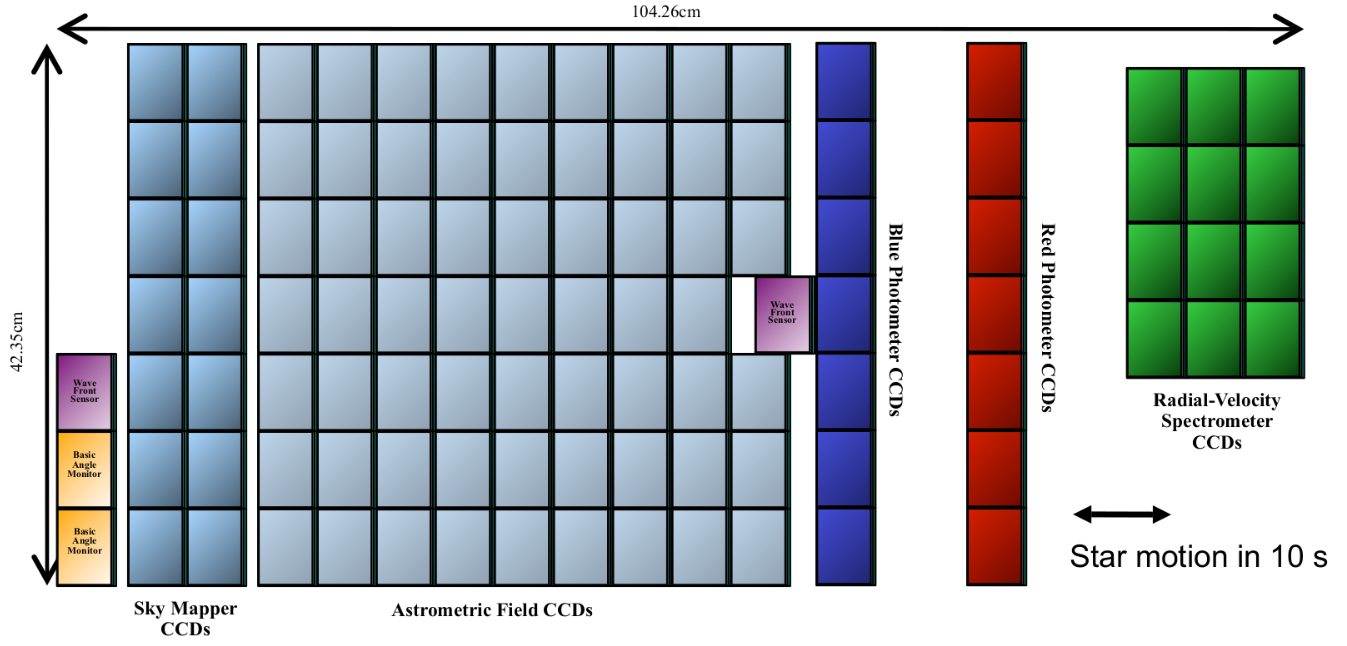
\includegraphics[width=0.9\linewidth]{Chapter4/gaia_detect_edit.png}
%     \caption[Schema of the \Gaia~detector]{Schematic diagram of the \Gaia~focal plane consisting of 106 CCDs, with the positions and dedicated instrument allocation of individual CCD modules annotated. Credit: ESA - A. Short}
%     \label{fig:gaia_focalplane}
% \end{figure}

\subsection{Astrometry}
The second data release for the \Gaia~mission, Gaia DR2 (hereafter DR2), occurred in April 2018 \citep{gaia_collaboration_gaia_2018}. It contained five-parameter astrometric solutions ($\alpha$, $\delta$, $\mu_{\alpha^*}$, $\mu_{\delta}$, $\pi$) for 1.7\,billion stars, combined with photometric and spectrometric (G, G$_{BP}$, G$_{RP}$) magnitudes for 1.3\,billion stars. \citet{bailer-jones_estimating_2018} computed geometric distance estimates for all stars with a parallax in the DR2 release. These distances were calculated using an inference approach that included length scale priors based on 3D models of the Milky Way. This method allowed distances to be inferred for all stars, even for those with high parallax uncertainties, where the length scale prior dominated the distance determination. We use both of these data products for the following analysis.

\section{Clustering methods}
We investigated a number of algorithms to identify probable cluster members, including Mean-Shift Clustering, Density-based Spatial Clustering of Applications with Noise (DBSCAN), the Hierarchical variant of DBSCAN (HDBSCAN), and Expectation–Maximisation (EM) clustering using Gaussian Mixture Models (GMM). We provide a description of how these algorithms function below, and discuss the benefits and limitations of each. For each of these algorithms we examined subsets of DR2 dataset centred on the four open clusters in the \Kepler~FoV. We sought to assign membership scores for each star in these subsets, which can be simply a binary (yes/no) membership determination depending on the algorithm used. It should be noted that the HDBSCAN algorithm lacked a python implementation when this work commenced and so was not selected as the preferred analysis method. A python implementation is now available, so it is included in this comparison to show its potential for future cluster membership determination.

\subsection{Mean-Shift Clustering}

The mean-shift clustering algorithm \citep{comaniciu_mean_2002} locates local over-densities in N-dimensional data using a centroid-based, sliding window. The algorithm begins with a randomly-selected initialisation point at the centre of a radially-profiled kernel (e.g. circular window in 2-D) in the parameter space. This kernel is iteratively shifted to higher density regions by calculating the mean of all enclosed points. The iterative shifting is concluded when the total number of points within the window no longer increases and convergence is achieved. 

This process is repeated with additional kernels until every data point in the parameter space is contained within a window, and thus assigned to a particular cluster. If multiple windows overlap, the window with the greatest density is preserved as the parent cluster, and the remaining windows eliminated.

The primary benefit of the mean-shift clustering algorithm is its ability to locate clusters without prior knowledge of the number of clusters present. This is offset by the need to tune the kernel radius hyper-parameter, a task that may be non-trivial. This process returns a yes/no classification of cluster membership and does not account for data points that may not be related to any particular cluster (i.e. noise).

\vspace{10pt}

\noindent{\bf In summary:}

\noindent{\bf Pros}: 
\begin{itemize}
    \item Automatically determines the number of clusters, so no prior knowledge of clusters is required.
\end{itemize} 

\noindent{\bf Cons}: 
\begin{itemize}
    \item Selection/tuning of the kernel radius hyper-parameter can be non-trivial.
    \item Binary classification to a particular cluster only (member/non-member).
    \item Cannot account for stars that do not belong to any cluster (e.g. field stars).
    \item Cannot account for clusters of different densities.
    \item Does not include measurement uncertainties.

\end{itemize}

\subsection{Density-based Spatial Clustering of Applications with Noise (DBSCAN)}

DBSCAN is a classification algorithm designed to locate clusters of over-density within a given parameter space whilst accounting for the presence of non-members \citep{ester_density-based_1996}. These non-members are referred to as `noise' in data clustering terminology.

The algorithm selects an arbitrary initialisation point and calculates a distance metric for the given parameter space to all other data points. If there are at least \texttt{min\_points} within a given maximum separation, $\epsilon$, it classifies the point as belonging to a cluster, otherwise it is classified as a non-member. All data points within a distance $\epsilon$ of a cluster member are associated with the same cluster, and the classification is repeated iteratively until all points within the $\epsilon$ neighborhood of the cluster have been added. This process is repeated until all points have either been assigned to a cluster or classified as non-members.

DBSCAN's main advantage over mean-shift clustering is the ability to account for data that includes non-members where no cluster assignment is valid. It is also capable of locating clusters of arbitrary shapes and sizes. As with mean-shift clustering, DBSCAN has difficulty accounting for clusters of different densities, since the hyper-parameters will change from cluster to cluster. Tuning the hyper-parameters to account for normalised distances between parameter spaces can also be difficult, particularly with high-dimensional data.

\vspace{10pt}

\noindent{\bf In summary:}

\noindent{\bf Pros}: 
\begin{itemize}
    \item Automatically determines the number of clusters, so no prior knowledge of clusters is required.
    \item Can account for arbitrary cluster shapes and sizes.
    \item Can account for datasets that include non-members.
\end{itemize} 

\noindent{\bf Cons}: 
\begin{itemize}
    \item Selection/tuning of the distance, $\epsilon$, and minimum cluster members, \texttt{min\_points}, hyper-parameters can be non-trivial.
    \item Normalising dimensions, and thus calculating the $\epsilon$ hyper-parameter for high-dimensional data, can be difficult.
    \item Binary classification to cluster only (member/non-member).
    \item Cannot account for clusters of varied density.
\end{itemize}

\subsection{Hierarchical DBSCAN (HDBSCAN)}

HDBSCAN \citep{campello_density-based_2013} is a variation of the traditional DBSCAN algorithm. The algorithm begins by producing a new distance metric, known as a mutual reachability metric, to lower the effect of non-members preventing convergence of membership models, whilst retaining the true cluster density. It then iterates over decreasing minimal density values, based on the mutual reachability metric, required for cluster identification. The result of this iterative process is a minimum spanning tree of the data set for differing density values. The algorithm then condenses this tree based on a minimum cluster size, selecting those clusters that persist for the greatest range of density values as the clusters to be returned. 

The primary benefit of HDBSCAN is its ability to include differences in cluster densities, allowing the identification of multiple clusters with different densities. In addition, HDBSCAN is capable of locating clusters of arbitrary shapes, sizes and densities. This algorithm can be used to provide a measure of the likelihood of membership, based on the stability of the clusters in hierarchical clustering space. However, this can be difficult to convert to a membership probability, making tuning the membership cutoff a non-trivial problem. The ability of this algorithm to isolate cluster members from field contaminants also depends on the relative differences between the cluster and the field densities and locations in parameter space, resulting in some cases where a clean cluster membership determination is difficult to achieve.

\vspace{10pt}

\noindent{\bf In summary:}

\noindent{\bf Pros}: 
\begin{itemize}
    \item Automatically determines the number of clusters, so no prior knowledge of clusters is required.
    \item Can account for arbitrary cluster shapes and sizes.
    \item Can account for noisy data.
    \item Can account for clusters of varied density.
\end{itemize} 

\noindent{\bf Cons}: 
\begin{itemize}
    \item Selection/tuning of the minimum cluster size hyper-parameter can be non-trivial.
    \item Overlapping over-densities within parameter space can be difficult to isolate as separate clusters.
    \item Converting to a membership probability is difficult.
    \item Cannot account for uncertainties in measurement.
\end{itemize}

\subsection{Expectation-Maximisation (EM) using Gaussian Mixture Modelling (GMM)}

Gaussian mixture modeling (GMM) \cite[e.g.][]{mclachlan_finite_2004} is a clustering algorithm designed to efficiently identify over-densities in n-dimensional parameter spaces using a more flexible Gaussian kernel. A pre-selected number, \texttt{k}, of Gaussian kernels, greater than or equal to the number of clusters present, are randomly initialised in parameter space. The posterior probabilities of each data point belonging to the \texttt{k} Gaussian distributions are then calculated. 

The algorithm then shifts the Gaussian kernels to maximise the probabilities of the data points within each distribution, using the Expectation-Maximisation (EM) algorithm \citep{blei_variational_2005}. This maximisation is achieved by summing data point positions weighted by their posterior probabilities. This process is iteratively repeated until convergence. 

The primary benefit of GMMs is that the Gaussian kernels allow the membership probability of data points to be calculated with respect to a given distribution as a fractional value rather than a binary yes/no membership. This allows us to calculate the likelihood that a star belongs one possible cluster compared to another. Additionally, these kernels allow for much greater flexibility in fitting arbitrary n-dimensional cluster distributions. Since Gaussian kernels are relatively computationally inexpensive, this is also one of the fastest clustering algorithms.

\vspace{10pt}

\noindent{\bf In summary:}

\noindent{\bf Pros}: 
\begin{itemize}
    \item Posterior probability of membership allows us to compare the likelihood that a star belongs to specific clusters.
    \item Non-binary membership determination allows calculation of membership probability.
    \item Can account for non-circular cluster shapes and sizes.
\end{itemize} 

\noindent{\bf Cons}: 
\begin{itemize}
    \item Cannot determine the number of clusters automatically.
    \item Cannot account for noise in data set unless over-fitting.
\end{itemize}
%\subsection{More realistic modelling}

\subsection{Algorithm testing}

We tested each of the above four algorithms on the four open clusters in the \Kepler~field of view based on two sets of input parameters: (1) position and proper motion, and (2) position, proper motion, and parallax. To obtain the cleanest membership for each clustering method, we iterated over the input parameters for each clustering algorithm until the colour-magnitude diagram (CMD) of the member stars showed a clear isochrone with few outliers. The position of stars in the CMD was not used to determine the membership scores, but instead was used only as a visual check to ensure the cluster subset was clearly defined. These CMDs provide a qualitative method for determining cluster membership and it should be noted that this process is susceptible to bias.

\begin{figure}[hbtp]
    \centering
    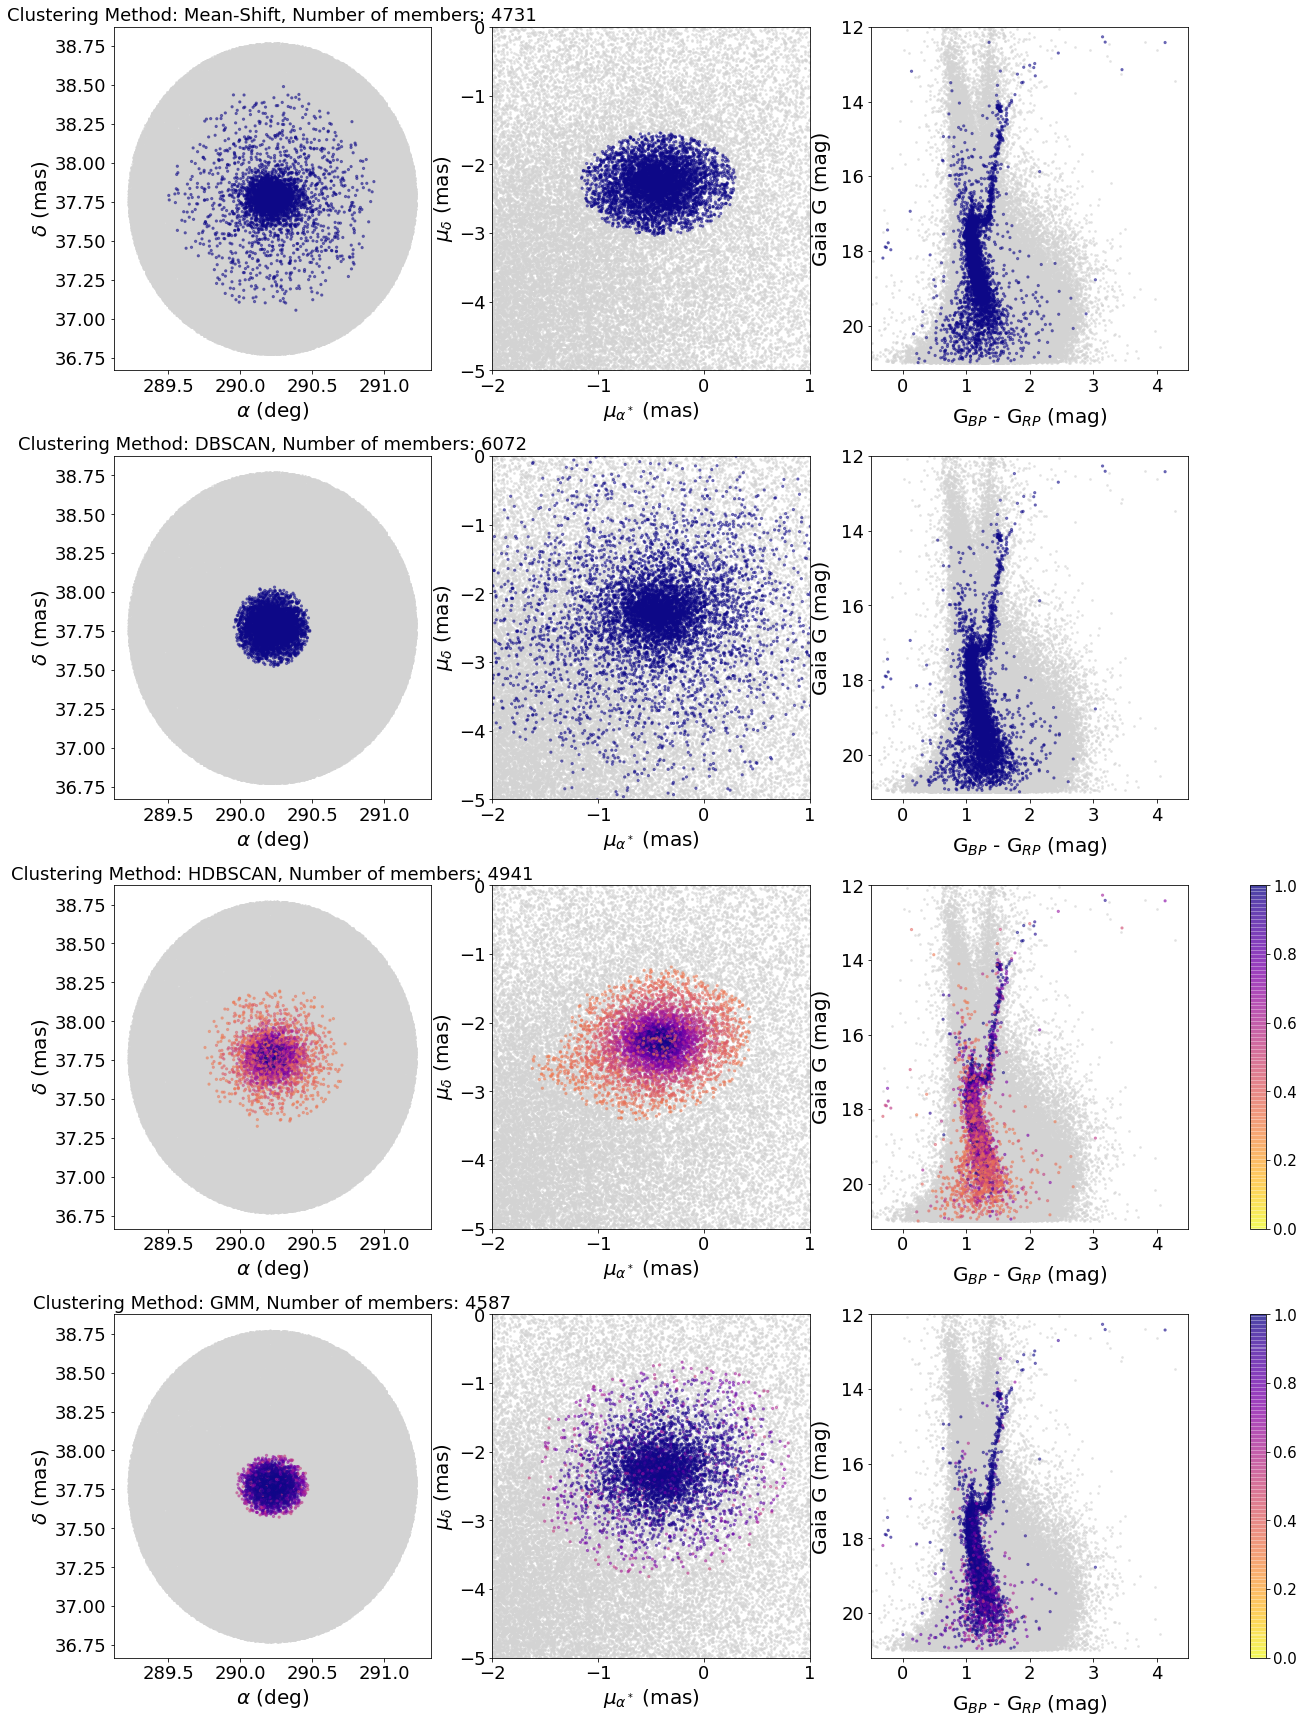
\includegraphics[width=0.92\linewidth]{Chapter4/6791_cluster_comp_pospm.png}
    \caption[Clustering method comparison - NGC\,6791 (I)]{Comparison of clustering methods used on NGC\,6791 using position and proper motion data. We plot cluster members (blue - binary identification, colour-coded - membership score) superimposed over the field stars (grey), with membership based on a single iteration of the clustering algorithm. We did not include measurement uncertainties in this algorithm testing, but include them in our final membership determinations.}
    \label{fig:clustering_methods_comparison_nopara}
\end{figure}

\begin{figure}[hbtp]
    \centering
    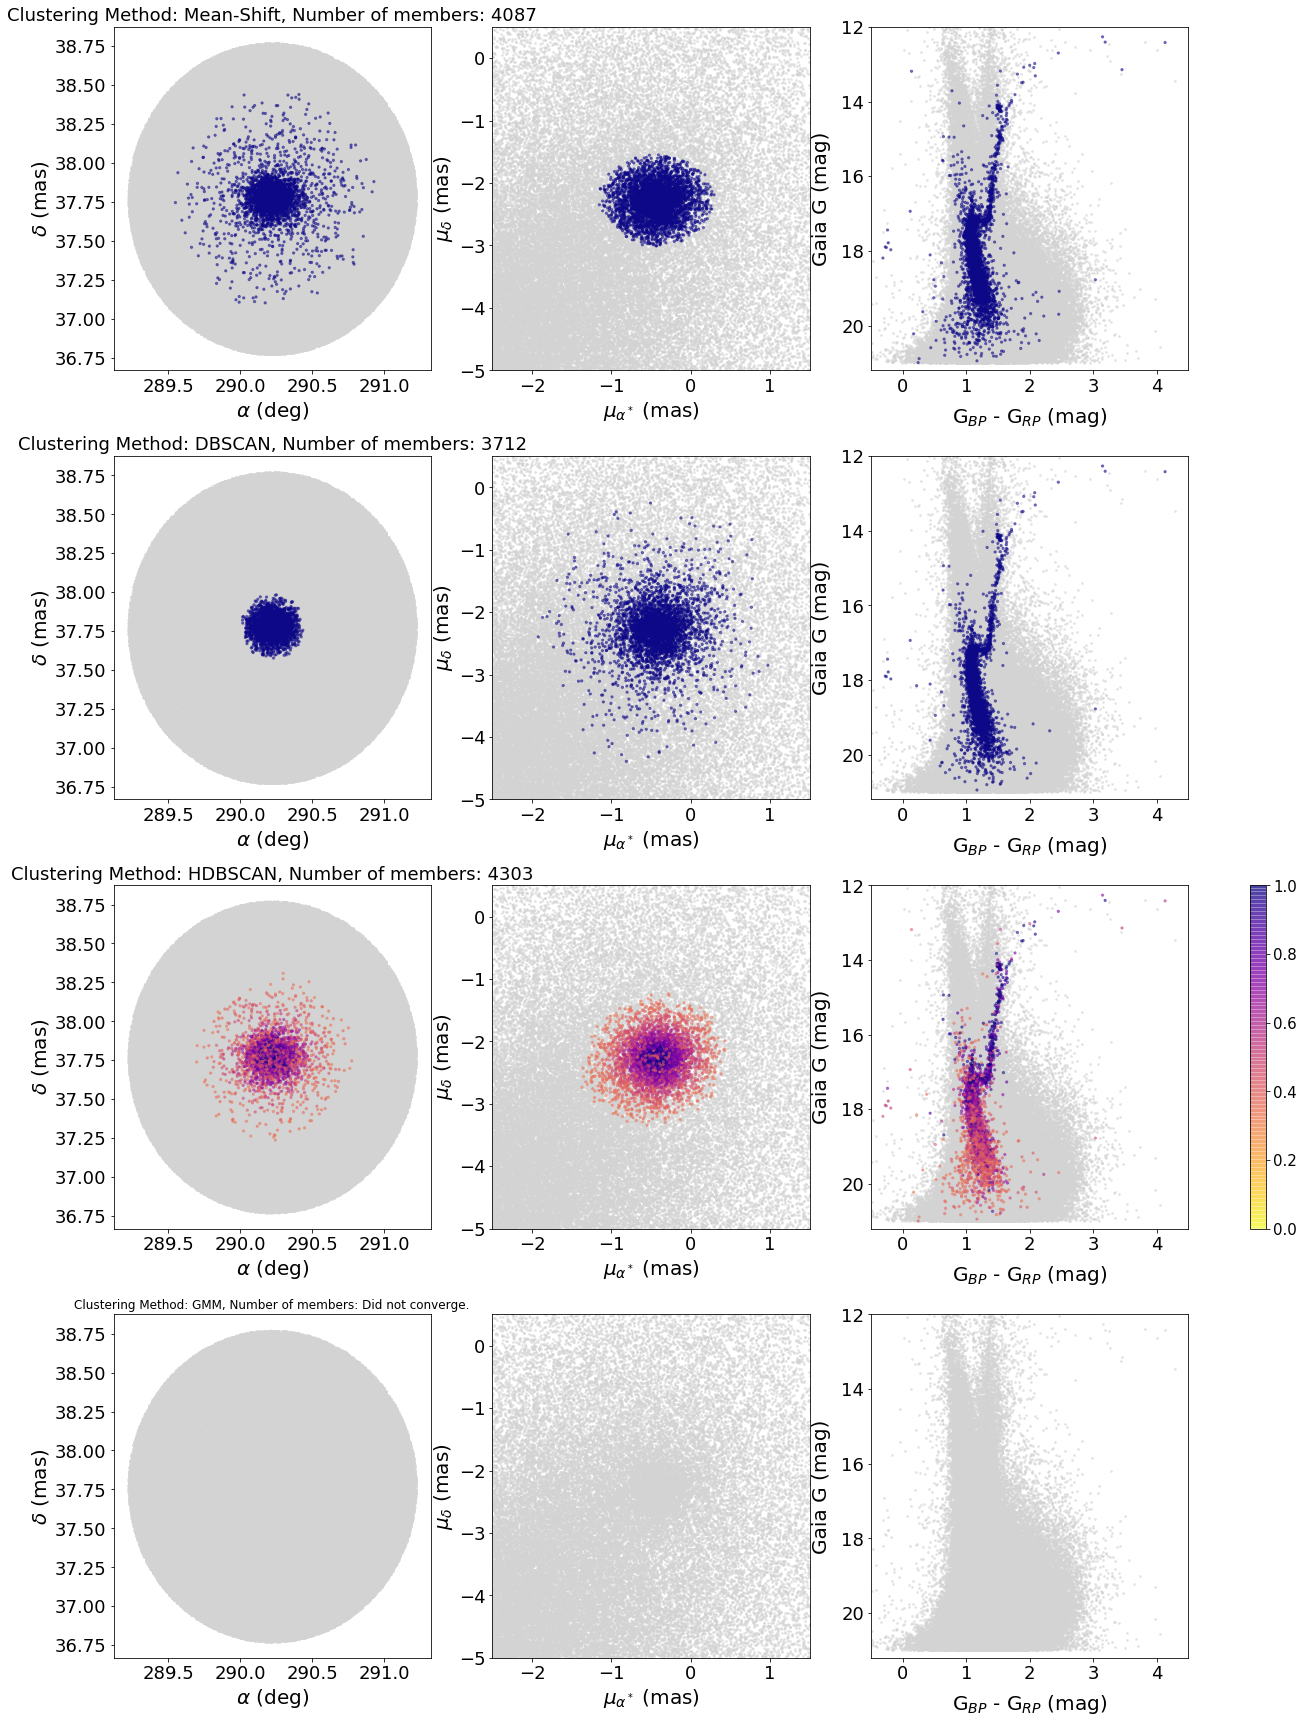
\includegraphics[width=0.92\linewidth]{Chapter4/6791_cluster_comp_pospmpara.png}
    \caption[Clustering method comparison - NGC\,6791 (II)]{Same as Figure \ref{fig:clustering_methods_comparison_nopara} but using position, proper motion, and parallax data.}
    \label{fig:clustering_methods_comparison_para}
\end{figure}

Figures \ref{fig:clustering_methods_comparison_nopara} and \ref{fig:clustering_methods_comparison_para} present the resulting cluster membership determinations for NGC\,6791. Figure \ref{fig:clustering_methods_comparison_nopara} is based solely on position and proper motion of the stars, whilst Figure \ref{fig:clustering_methods_comparison_para} also includes stellar parallax. From top to bottom, the rows present the clustering results from Mean-Shift, DBSCAN, HDBSCAN, and GMM clustering algorithms. The HDBSCAN algorithm was not available as a public package until after the analysis contained herein was complete. We provide its inclusion here as a reference to show its potential benefits for improving future membership studies. Field stars (grey) are over-plotted with likely cluster member stars (blue for binary membership determination, and coloured points for fractional membership score). In those cases where only grey points are shown, we were unable to find input parameters for the clustering algorithm that converged to the cluster member stars. Determining optimal hyper-parameters for each clustering algorithm is time-consuming so we have produced this comparison only for NGC\,6791. We use this cluster as the test case for selecting the algorithm to be used for the proceeding analysis. Whilst the global properties of the clusters differ, their members have mean values and distributions that differ from their surrounding field star populations, and it is this distinction that our clustering analyses depend upon. The algorithm hyperparameters for different clusters will reflect their specific global properties, but does not have a major impact on the clustering method itself and so does not play a big role in algorithm selection.

The inclusion of parallax values produces cluster CMDs that have narrower main sequences and fewer outliers from the cluster isochrone for fainter stars. This indicates that these outliers are likely non-member stars in the foreground or background that have similar proper motions to the cluster members. Whilst a comparison between these figures reveals the apparent benefit of including parallax measurements in the clustering analysis, we decided against their inclusion in our final membership determination. We made this decision as we prioritised having fractional membership scores, rather than a member/non-member determination, over a potential improvement in membership determination that was restricted only to fainter stars. This necessitated the use of the GMM algorithm for which no convergence to a cluster population was reached when parallax measurements were included. We note that for brighter members the inclusion of parallax affected the membership for only a very small number of stars in the clustering algorithms that converged. Furthermore, both NGC\,6791 and NGC\,6819 are distant clusters, resulting in large uncertainties on the parallax measurements that are propagated through our analysis, and result in large uncertainties in the cluster membership values.

% \todo{COMPLETE THE IMAGES FOR THIS SECTION AND FOR THE APPENDICES FOR 6819, 6866, 6811}

\section{Membership}

The main aim of this work is to provide membership scores for all stars in the open clusters located in the nominal \Kepler~FoV. We are primarily focused on NGC\,6791 and NGC\,6819, with the aim to identify cluster members so the \Kepler~data of these stars can be extracted from the superstamps (see \cref{chap:intro:data}) for ensemble analysis. The other two clusters are included for completeness.

We selected the Gaussian Mixture Modelling (GMM) clustering algorithm primarily based on its ability to provide a fractional membership score for all stars, compared to the member/non-member determination returned by the DBSCAN and Mean-Shift algorithms. A secondary consideration was the fast computational speed of the GMM algorithm, which enabled extensive sampling of the uncertainty parameter space to be completed in a realistic time frame. We also considered the ease of hyperparameter tuning with a focus on the need to re-tune these parameters as we sampled the uncertainty parameter space.

We used GMM to calculate the membership score for all stars within selected radii of the four open clusters in the nominal \Kepler~field of view. We initially selected these radii to be approximately 2.5 times the published radii for the larger clusters of NGC\,6791 and NGC\,6819, and 4 times the reported radii for the smaller clusters of NGC\,6811 and NGC\,6866, to ensure no potential cluster members were missed. The published radii were all extracted from radial stellar density profiles that were calculated from 1 arcsecond concentric annuli around the cluster centres. Different models were fit to these density profiles making a direct comparison between the radii difficult, however, our membership analysis shows all members well within the selected cone search radii. The smaller clusters were reprocessed for all clustering methods after the HDBSCAN algorithm became available to ensure that the selected radii were larger than the maximum distance of possible cluster members retrieved using the HDBSCAN algorithm. Table \ref{tab:cluster_selection} presents the positions and final radial distance cuts we used for each cluster.

We downloaded \Gaia~DR2 data for all stars within the radial distance cut of the cluster centres to ensure our membership determination was as complete as possible. 
NGC\,6791 and NGC\,6819 are both distant clusters (see \cref{tab:cluster_properties}) with most cluster members being much fainter than the field stars. \cite{lindegren_gaia_2018} determined that the typical astrometric uncertainty for stars of magnitude $G=17$ is at least twice as high as those with $G<14$\,mag and suggested photometric cuts that bias against fainter stars to ensure high quality astrometric solutions. Since these clusters have many faint members we make no magnitude cuts at this point despite the significant decrease in astrometric quality for stars fainter than $G=17$\,mag. We have excluded radial velocity measurements from our analysis because these are only available for a small fraction of stars, with almost none of the cluster members from NGC\,6791 having such values. Similarly, we did not include parallax values in our clustering analysis because the values are very small (distances are $\sim$2 \& $\sim$4\,kpc, respectively), resulting in very large relative uncertainties.

\begin{savenotes}
\begin{table}[!t]
    \centering
    \setlength\tabcolsep{10pt}
    \begin{tabular}{ccccc}
        \hline
        Cluster     & RA        & Dec       & Radius    & Radial distance \\
                    & (deg)     & (deg)     & (arc mins) & cut (arc mins) \\
        \hline
        \hline
        NGC 6791    & 290.2208  & 37.771    & 15.0\footnote[1]{\citep{platais_new_2011}} & 60.0\\
        NGC 6819    & 295.325   & 40.1867   & 15.0\footnote[2]{\cite{sagar_study_2002}} & 48.0\\
        NGC 6811    & 294.3208  & 46.3883   & 3.0\footnote[3]{\cite{sagar_study_2002}} & 28.0\\
        NGC 6866    & 300.9792  & 44.1583   & 7.5\footnote[4]{\cite{sagar_study_2002}} & 52.0\\
        \hline
    \end{tabular}
    \caption[Cluster positions and radial cuts]{Positions and angular size of the open clusters in the \Kepler~FoV and the radial distance cut used for each cluster for determining the probability of cluster membership.}
    \label{tab:cluster_selection}
\end{table}
\end{savenotes}

%\vspace{3pt}

We used the position ($\alpha$, $\delta$) and proper motion ($\mu_{\alpha}$, $\mu_{\delta}~cos\delta$) parameter space for all \Gaia~sources within the cutoff radius in our Gaussian Mixture Modelling analysis. %\todo{citation} 
Godoy-Rivera (2019 in prep.; priv. comm.) note that clustering methods fail to converge when including stars that are at large radial distances from the cluster centre as a result of the field population dominating the fit. To account for this, we over-fitted the field component using multiple Gaussian kernels. We selected the optimum kernel number by running initial GMM analyses on each data set, iteratively increasing the number of kernels used, until the subset of stars classified as cluster members showed a clear empirical isochrone upon visual inspection of the observational colour-magnitude diagram corresponding to their colours and magnitudes. 

% Until population of stars assigned to the Gaussian component corresponding to the cluster members forms an empirical isochrone in the observational CMD.
Once the hyper-parameter for the optimum number of Gaussian kernels was set, we repeated the GMM analysis using a Monte Carlo simulation, with random Gaussian noise added to each data point based on the uncertainties of the \Gaia~measurements ($\sigma_{\mu\alpha}$, $\sigma_{\mu\delta}$, $\sigma_{\alpha}$, $\sigma_{\delta}$). We included this process to sample the uncertainty parameter space and determine the membership score distribution. This allowed us to account for the heteroskedastic data in our membership analysis. For each iteration of the Monte Carlo simulation, we accepted the solution if at least half the stars classified as members in the initial run were also classified as members in the current run, otherwise we rejected the solution. We repeated this process until a minimum of 1000 successful convergences were recorded for each open cluster data set. We assumed no covariance between the \Gaia~uncertainties, however, it would be more rigorous to include these in the Monte Carlo sampling given the resulting membership score distributions may be biased towards less likely parameter combinations. This will be a key point for improving upon these results in future analyses.

To select likely cluster members we applied cuts (see \cref{tab:cluster_crossmatch}) to the GMM membership score distributions based on their mean and standard deviations. For example, we applied a cut of 0.03 in the mean membership score for NGC\,6791 and NGC\,6819 based on visual inspections of the resulting CMD, with the cut selected to produce a visually clean CMD. To exclude any stars that are foreground contaminants for NGC\,6791 and NGC\,6819 we applied a further minimum distance cut of 2000\,pc and 800\,pc, respectively, based on the \cite{bailer-jones_estimating_2018} `$\texttt{r\_lo}$' values. The $\texttt{r\_lo}$ and $\texttt{r\_hi}$ values in this catalog present the equivalent of a 1-$\sigma$ uncertainty on the distance given the non-Gaussian and asymmetric posterior probability distributions on the parallax to distance conversion. % correspond to the lower and upper boundaries, respectively, of the highest posterior probability for distance with an integral probability of \~68\%. 
We applied tighter distance constraints to the closer clusters of NGC\,6811 and NGC\,6866 due to the lower uncertainty on the likely cluster member parallax values (used to calculate the distances). For NGC\,6811 we set `$\texttt{r\_lo}$' $\leq 1400$\,pc and `$\texttt{r\_hi}$' $\geq 1000$\,pc to prevent the moderately rich field population \citep{janes_open_2014} from affecting our clustering analysis by creating a rare case classification problem. For NGC\,6866, located in the lowest field population region of the four clusters, the constraints we used were `$\texttt{r\_lo}$' $\geq 800$\,pc and `$\texttt{r\_hi}$' $\geq 1300$\,pc.

After these cuts, we identify 2388 members for NGC\,6791, 3254 members for NGC\,6819, 393 members for NGC\,6811, and 483 members for NGC\,6866. Figures \ref{fig:cmd6791} to \ref{fig:cmd6866} show colour-magnitude diagrams for all four clusters, with field stars shown in light grey. 

NGC\,6791 and NGC\,6819 both have superstamp data of the crowded cluster centres. One of our primary goals in conducting this membership analysis was to extract data for non-targeted cluster members from the superstamp data to enhance the ensemble asteroseismic analyses of the clusters. The likely cluster members have therefore been divided into two subsets: those that fall outside the superstamp area (dark-grey), and those that fall within the superstamps (coloured by membership score). Our catalog contains the full set of membership scores for all stars, but we do not show these here to enable easy identification of those stars we wish to investigate further. For the red giant branch and blue straggler regions of these CMDs the likely members falling on silicon have been further divided. We have identified non-targeted stars from the \Kepler~mission (red circles), targeted blue straggler candidates (green circles), and red giants that were targeted for less than 9 quarters of the \Kepler~mission (blue circles). 

Neither NGC\,6811 or NGC\,6866 have superstamp data so for these clusters we do not subdivide the member stars, but rather plot all likely members colour-coded by membership score, with all targeted cluster members (green circles) identified. We can see that the initial selection functions for cluster members were essentially complete to $G\leq16.0$ for NGC\,6811, and to $G\leq14.0$ for NGC\,6866.

\begin{figure}[hbtp]
\centering
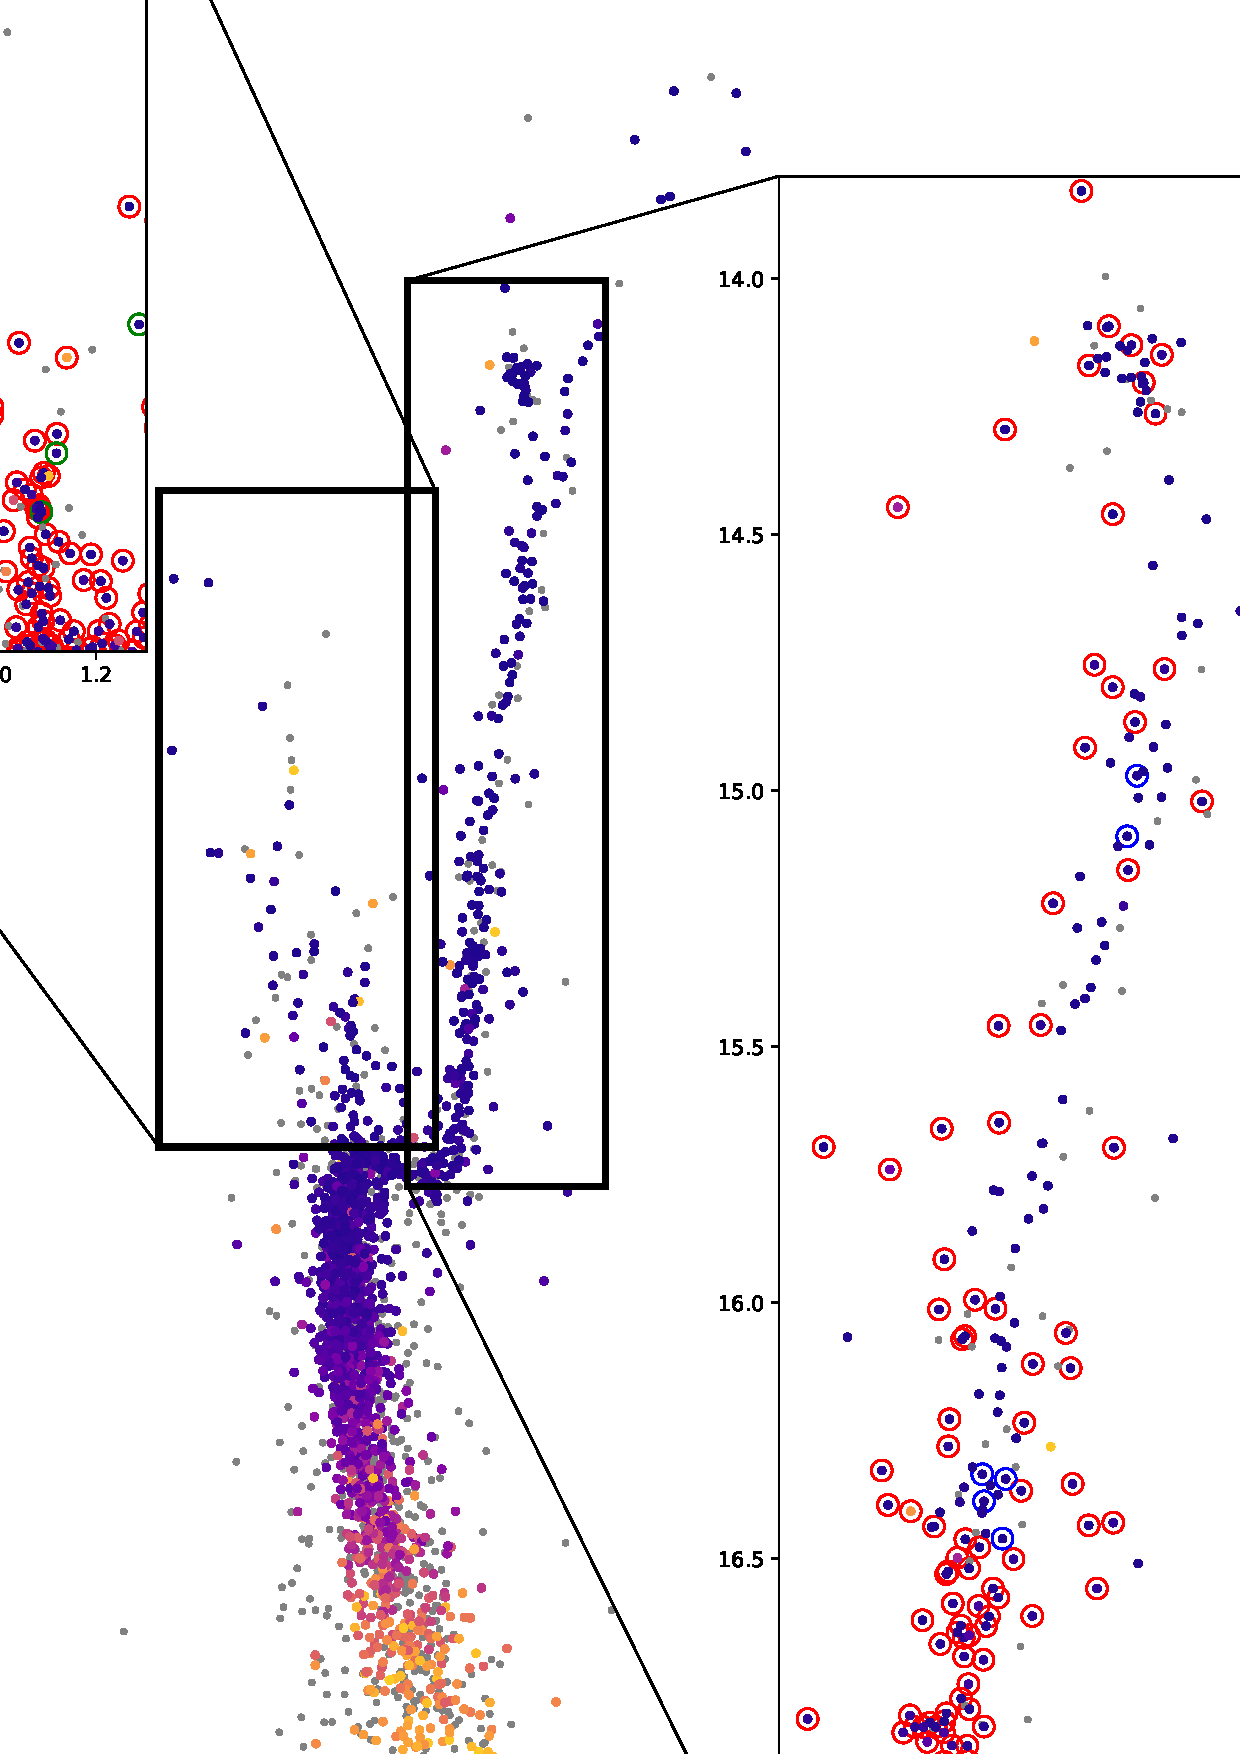
\includegraphics[width=\linewidth]{Chapter4/cmd_6791.jpg}
\caption[NGC\,6791 CMD]{Colour magnitude diagram of NGC\,6791 based on \Gaia{} photometry, showing field stars (light grey), and likely cluster members (dark grey) with those that fall inside the \Kepler~superstamps shaded by their mean membership score. For the red giant branch (right inset) and blue straggler stars (left inset) we have further highlighted the non-targeted superstamp stars (red circles, both), red giants observed for less than nine quarters (blue circles, right), and targeted blue stragglers (green circles, left)} % posterior_prob >= 0.03, stddev_posterior_prob <= 0.3
\label{fig:cmd6791}
\end{figure}

\begin{figure}[hbtp]
\centering
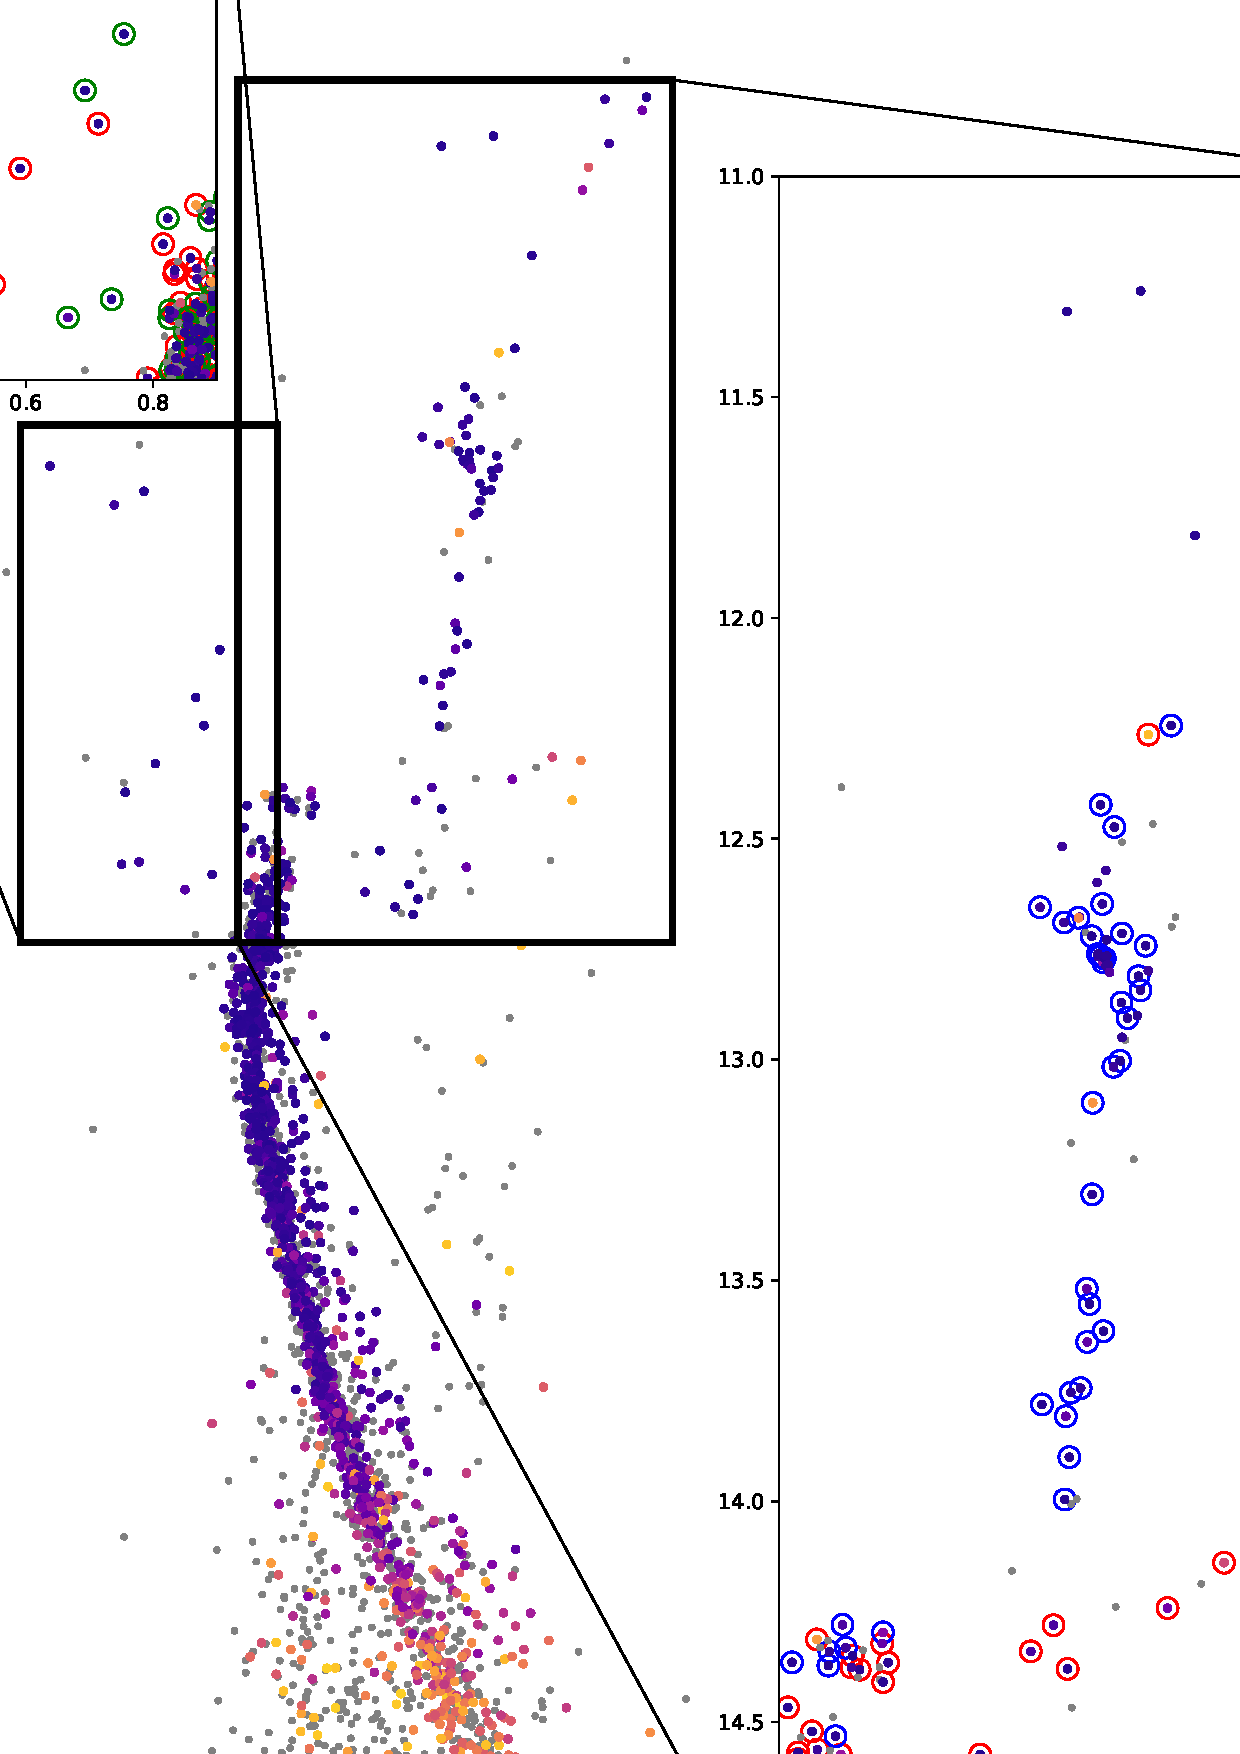
\includegraphics[width=\linewidth]{Chapter4/cmd_6819.jpg}
\caption[NGC\,6819 CMD]{Same as Figure \ref{fig:cmd6791} but for NGC\,6819.} % posterior_prob >= 0.03, stddev_posterior_prob <= 0.3
\label{fig:cmd6819}
\end{figure}

\begin{figure}[hbtp]
\centering
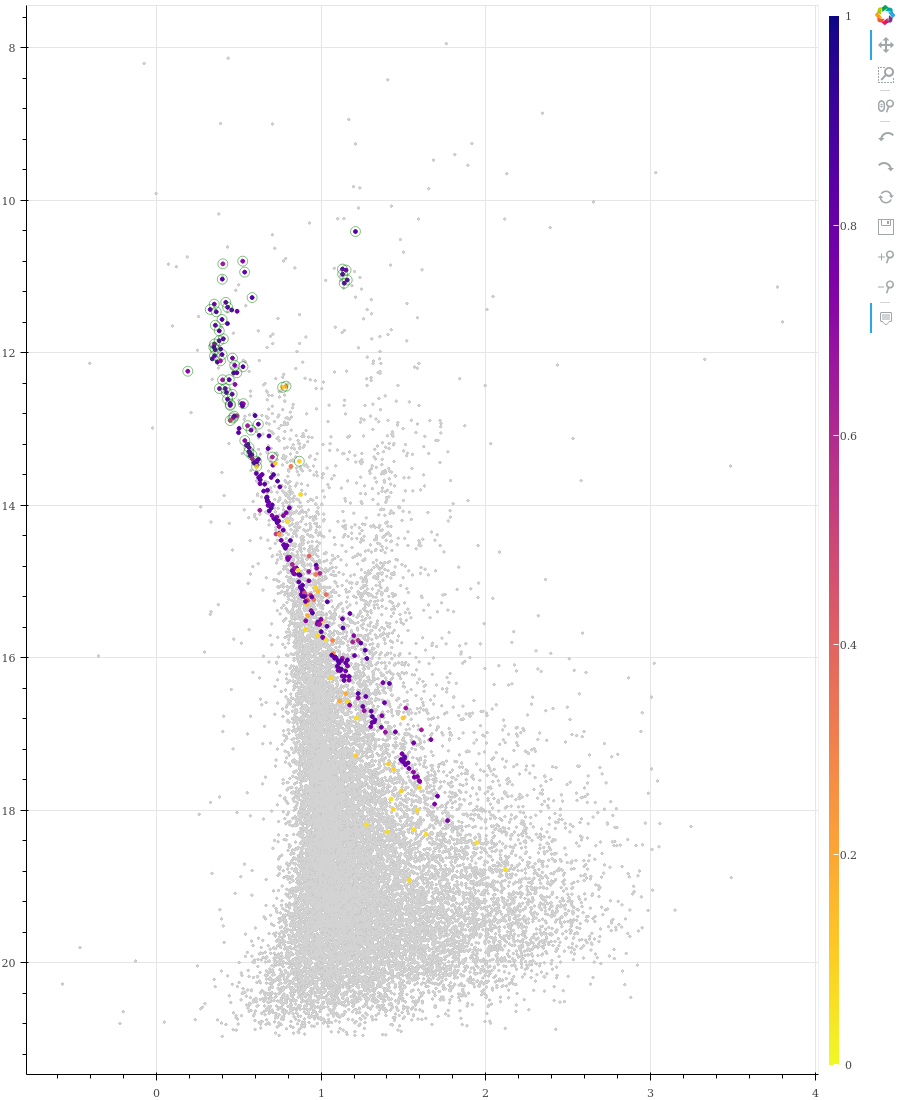
\includegraphics[width=\linewidth]{Chapter4/cmd_6811.jpg}
\caption[NGC\,6811 CMD]{Colour magnitude diagram of NGC\,6811 based on \Gaia{} photometry, showing field stars (light grey) and likely members shaded by their mean membership score. \Kepler~targeted stars (green circles) are highlighted. There are no superstamp images of this cluster.}
\label{fig:cmd6811}
\end{figure} % posterior_prob >= 0.05, stddev_posterior_prob <= 0.15

\begin{figure}[hbtp]
\centering
\includegraphics[width=\linewidth]{Chapter4/cmd_6866.jpg}
\caption[NGC\,6866 CMD]{Same as Figure \ref{fig:cmd6811} but for NGC\,6866}
\label{fig:cmd6866}
\end{figure} % posterior_prob >= 0.05, stddev_posterior_prob <= 0.15
\newpage

\section{Comparison with other surveys}
\subsection{Cantat-Gaudin (2018)}

CG18 conducted a membership analysis for every detected cluster in the whole-sky \Gaia~DR2 astrometric data, using a k-means-based minimal spanning tree to determine cluster membership. Their analysis was based on proper motion and parallax data, with ten iterations over the uncertainty parameter space to provide membership probability, compared to our Gaussian Mixture Model method based on proper motion and spatial data. CG18 were concerned with a large-scale automated membership analysis of every open cluster in \Gaia~DR2. We expect that analysing clusters with individually optimised parameters will allow for a more targeted, rigorous membership determination.

We note that CG18's membership probabilities for the four \Kepler~clusters do not include any stars they categorised as non-members (P$_{memb} = 0$). To account for this, we replicated the extraction procedure in CG18 to obtain their complete sample, selecting only stars with proper motions within 2\,mas\,yr$^{-1}$ of the identified over-density, and parallaxes within 0.3\,mas of the cluster. We used the computed median $\mu_{\alpha^{*}}$, $\mu_{\delta}$, and $\varpi$ of the probable cluster members reported in CG18 to specify these limits. We note that, despite CG18 detailing a tighter proper motion constraint of 0.5\,mas\,yr$^{-1}$ for some clusters more distant than 900\,pc, an inspection of the proper motion values for all of the cluster members in NGC\,6791 and NGC\,6819 revealed values up to double this limit. We assigned CG18 membership probabilities of 0 to any stars within these selection cuts that did not also appear in their membership lists.

\subsubsection{NGC 6791}

We have compared our membership values with those derived by CG18 for NGC\,6791 and have determined that they are mostly in agreement (see \cref{fig:CG_6791_comparison}). The small-number statistics of the bins where P$_{\rm memb}$ is between 0.1 and 0.7 probably account for the significant scatter from a linear relationship.

\begin{figure}[hbtp]
    \centering
    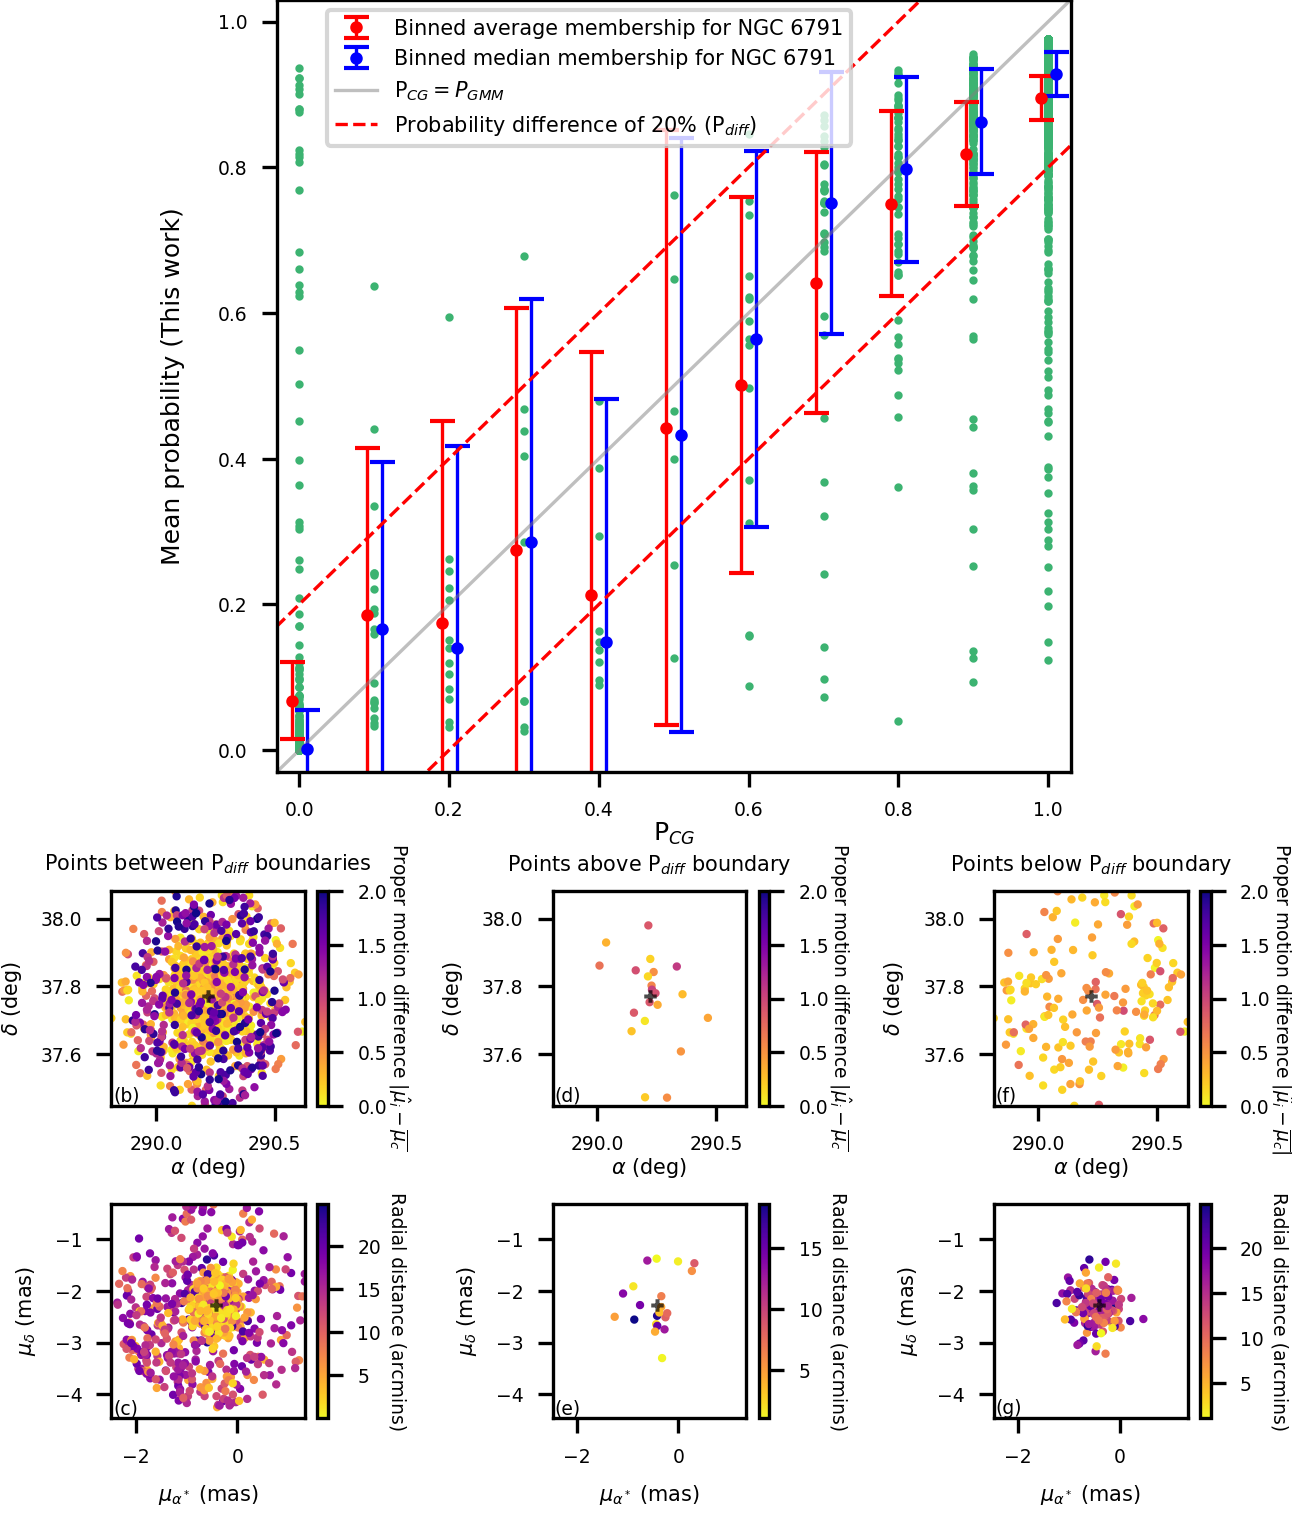
\includegraphics[width=0.95\linewidth]{Chapter4/NGC6791_CG_comparison_mod.png}
    \caption[Comparison of membership probabilities for NGC\,6791]{Comparison of membership probabilities between \cite{cantat-gaudin_gaia_2018} and this work for commonly investigated stars in NGC\,6791. (Top) The mean (red) and median (blue) of the membership distribution determined in this work for each bin corresponding to \cite{cantat-gaudin_gaia_2018}. The error bars correspond to the $1/\sqrt{\rm N}$ values for each bin and the mean and median values have been offset by $P_{\rm CG} \pm 0.01$ for visibility of the individual star membership values. The interval corresponding to $\pm$ 20\% difference in membership values (dashed red lines) is highlighted, with the stars within this boundary shown in (b) \& (c), those above shown in (d) \& (e), and those below shown in (f) \& (g). The membership outliers are plotted in terms of their position distributions (d, f), colour-coded by the quadrature of their proper motion difference from the average cluster proper motion, and in proper motion distributions (e,g), colour-coded by their angular separation from the cluster centre. The black crosses mark the cluster centres and mean cluster proper motions.}
    \label{fig:CG_6791_comparison}
\end{figure}

There are some outliers above and below the linear trend that show significant disagreement with our membership determination. We inspected the spatial and proper motion distributions of the 203 outliers ($\sim$11\% of the total comparison population) where the CG18 probability is at least 20\% lower than our membership value (Figure \ref{fig:CG_6791_comparison} (d) \& (e)), and at least 20\% higher than our membership value (Figure \ref{fig:CG_6791_comparison} (f) \& (g)). Of particular note are the 108 stars CG18 classified as definite members of the cluster where our method predicted membership scores below 80\%. These stars account for more than 50\% of the points in panels (f) and (g). One of the potential reasons for this disagreement is that the \textsc{Upmask} code used by CG18 does not account for field stars in the membership probability determination. For stars with a P$_{\rm memb} \geq 0.8$ in CG18, this missing field component can explain the artificially higher membership probabilities, but it does not account for the large spread in our membership values.

Figure \ref{fig:CG_6791_comparison} (f) and (g) reveal that for most of these outliers there is a tendency for stars at greater angular separations from the cluster to have smaller deviations in their proper motion vector relative to the cluster. We attribute our lower membership score for these likely cluster members to the Gaussian kernels we use for clustering. These kernels exhibit sharp cutoffs at the cluster's edges within the parameter space. Our lower determinations for these stars' membership scores are therefore expected as the spanning tree model used by CG18 is far more lenient for stars at the edges of the cluster's parameter space.

The outliers in Figure \ref{fig:CG_6791_comparison} (d) and (e), where we determined the membership score to be at least 20\% higher than CG18, show no trend in spatial distribution relative to their motion. Based on the \cite{bailer-jones_estimating_2018} distance cuts that we made for probable members above, a little under half of these outliers are likely to be foreground contaminants. For the remainder we attribute the difference to the different clustering algorithms applied, specifically the density hyper-parameter in the k-means algorithm.

\subsubsection{NGC 6819}

Our membership determinations for NGC\,6819 (Fig. \ref{fig:CG_6819_comparison}) show significant differences to those determined by CG18, with our values being lower by at least 15\%. The most likely explanation for this comes from the membership methods: our Gaussian Mixture Model provides a membership score as a normalised fraction of the cluster population to the combined cluster and field populations, whilst the minimal spanning tree used by CG18 accounts for no contribution to the membership probability from the field population.  Our comparison also relies on an accurate selection of the original \Gaia{} subset CG18 analysed to recreate the CG18 $P_{\rm memb} = 0$ population that were not included in their database. Despite our attempt to accurately recreate these subsets for each cluster it is possible that at least some stars with high membership scores from our analysis that fall in the $P_{\rm memb} = 0$ bin may include stars that were not actually analysed by CG18. This would artificially inflate the proportion of stars with highly differing membership values, and in future would be better addressed by obtaining the actual subset analysed by CG18.

NGC\,6819 is much closer to the Galactic plane and, as such, will have a much higher field contamination. This is a slightly non-linear effect across the spatial dimension of the cluster that scales in proportion to the density profile of the disk of the Milky Way in this same region. To apply a direct comparison we would need to determine the stellar density profile of the Milky Way and decrease the CG18 $P_{\rm memb}$ values accordingly for every star. This is beyond the scope of this work.

There are a number of stars we classify as having much higher membership scores than CG18. This difference is based primarily on the inclusion of the parallax values in CG18's analysis. We elected to not include parallax in our analysis of NGC\,6791 and NGC\,6819 as the 1-$\sigma$ and 3-$\sigma$ uncertainties, respectively for these clusters, is on the order of the parallax values themselves.

\begin{figure}[hbtp]
    \centering
    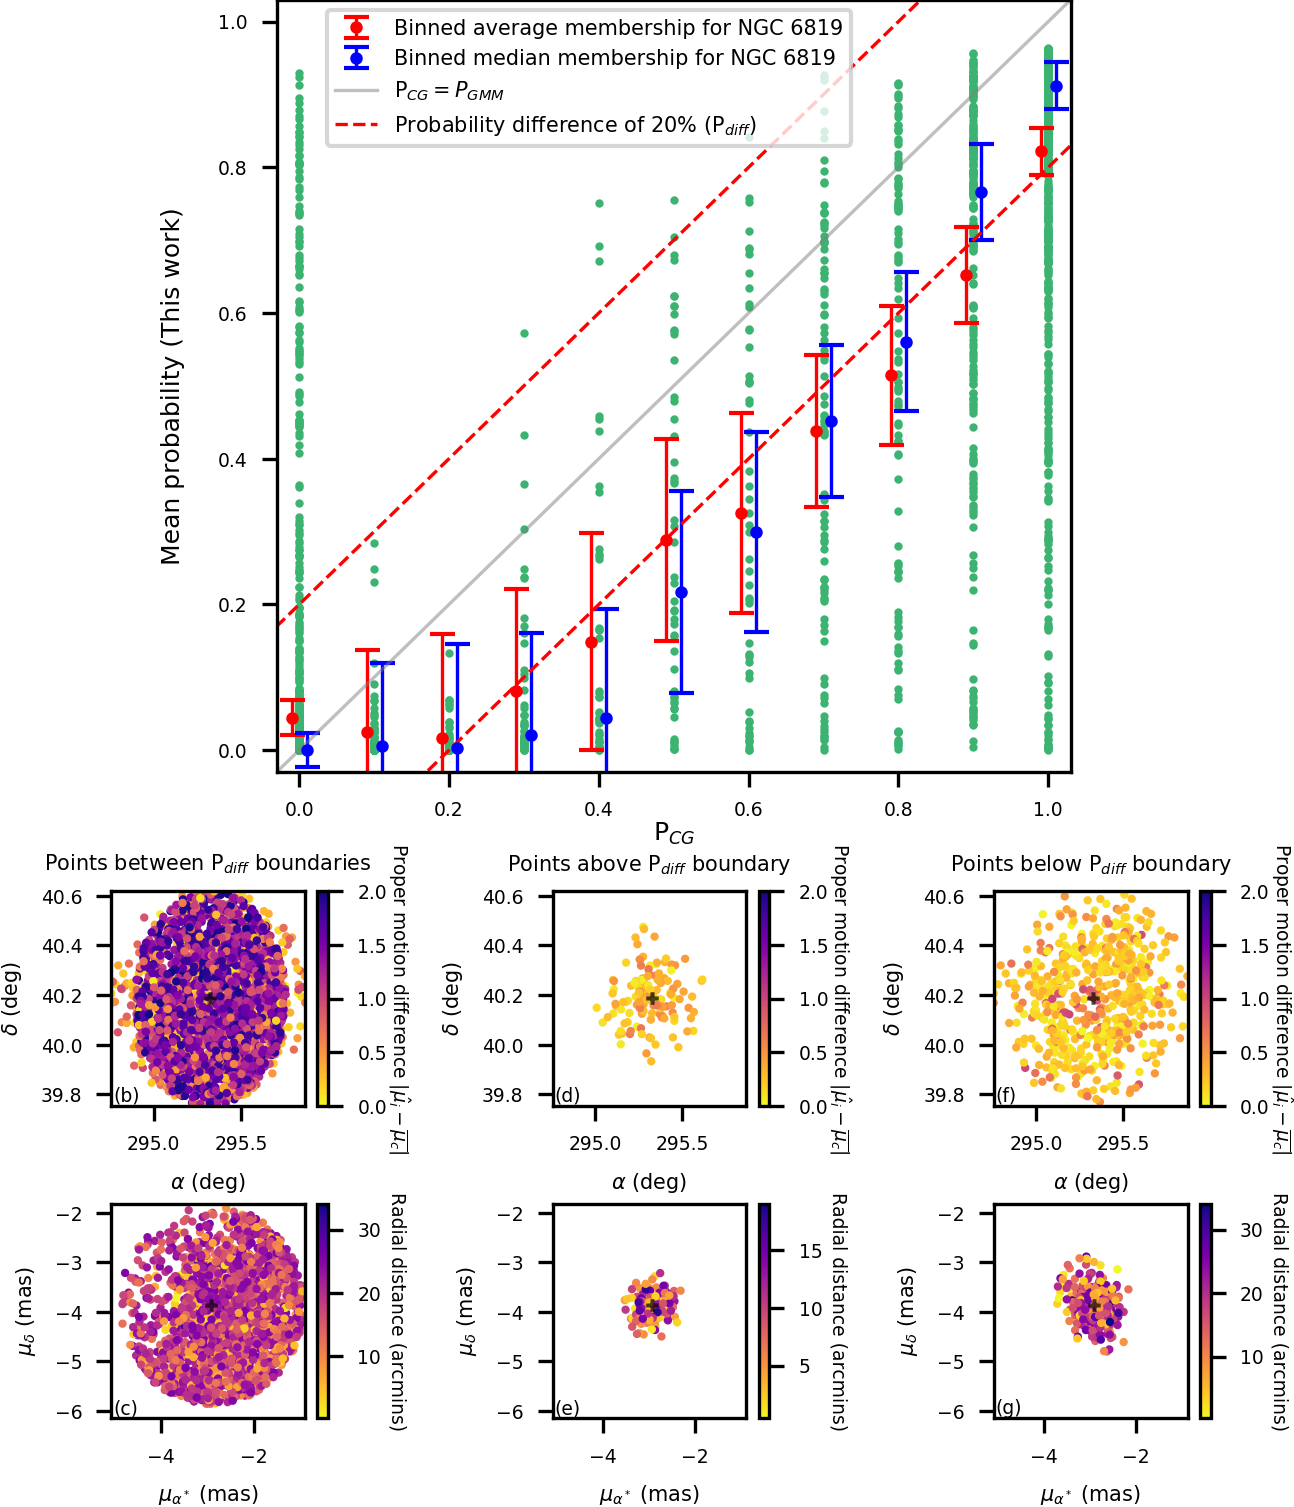
\includegraphics[width=\linewidth]{Chapter4/NGC6819_CG_comparison.png}
    \caption[Comparison of membership probabilities for NGC\,6819]{Same as Figure \ref{fig:CG_6791_comparison} but for NGC\,6819.}
    \label{fig:CG_6819_comparison}
\end{figure}

\subsubsection{NGC 6811 \& NGC 6866}

Figures \ref{fig:CG_6811_comparison} and \ref{fig:CG_6866_comparison} show the comparison between the membership probabilities of CG18 and our own for NGC\,6811 and NGC\,6866. We find significant deviations, following similar trends, between the membership probabilities of CG18 and our study for these clusters. As with NGC\,6819, deviations at higher CG18 membership probabilities are probably due to the normalisation applied by the GMM method to our membership scores that includes the distribution of the field stars. We note that our membership scores are significantly higher for stars CG18 classified as low probability members ($0.2 \leq $P$_{\rm memb} \leq 0.6$). As with NGC\,6791, the low number statistics in these membership bins dominates the mean and median values.

\begin{figure}[hbtp]
    \centering
    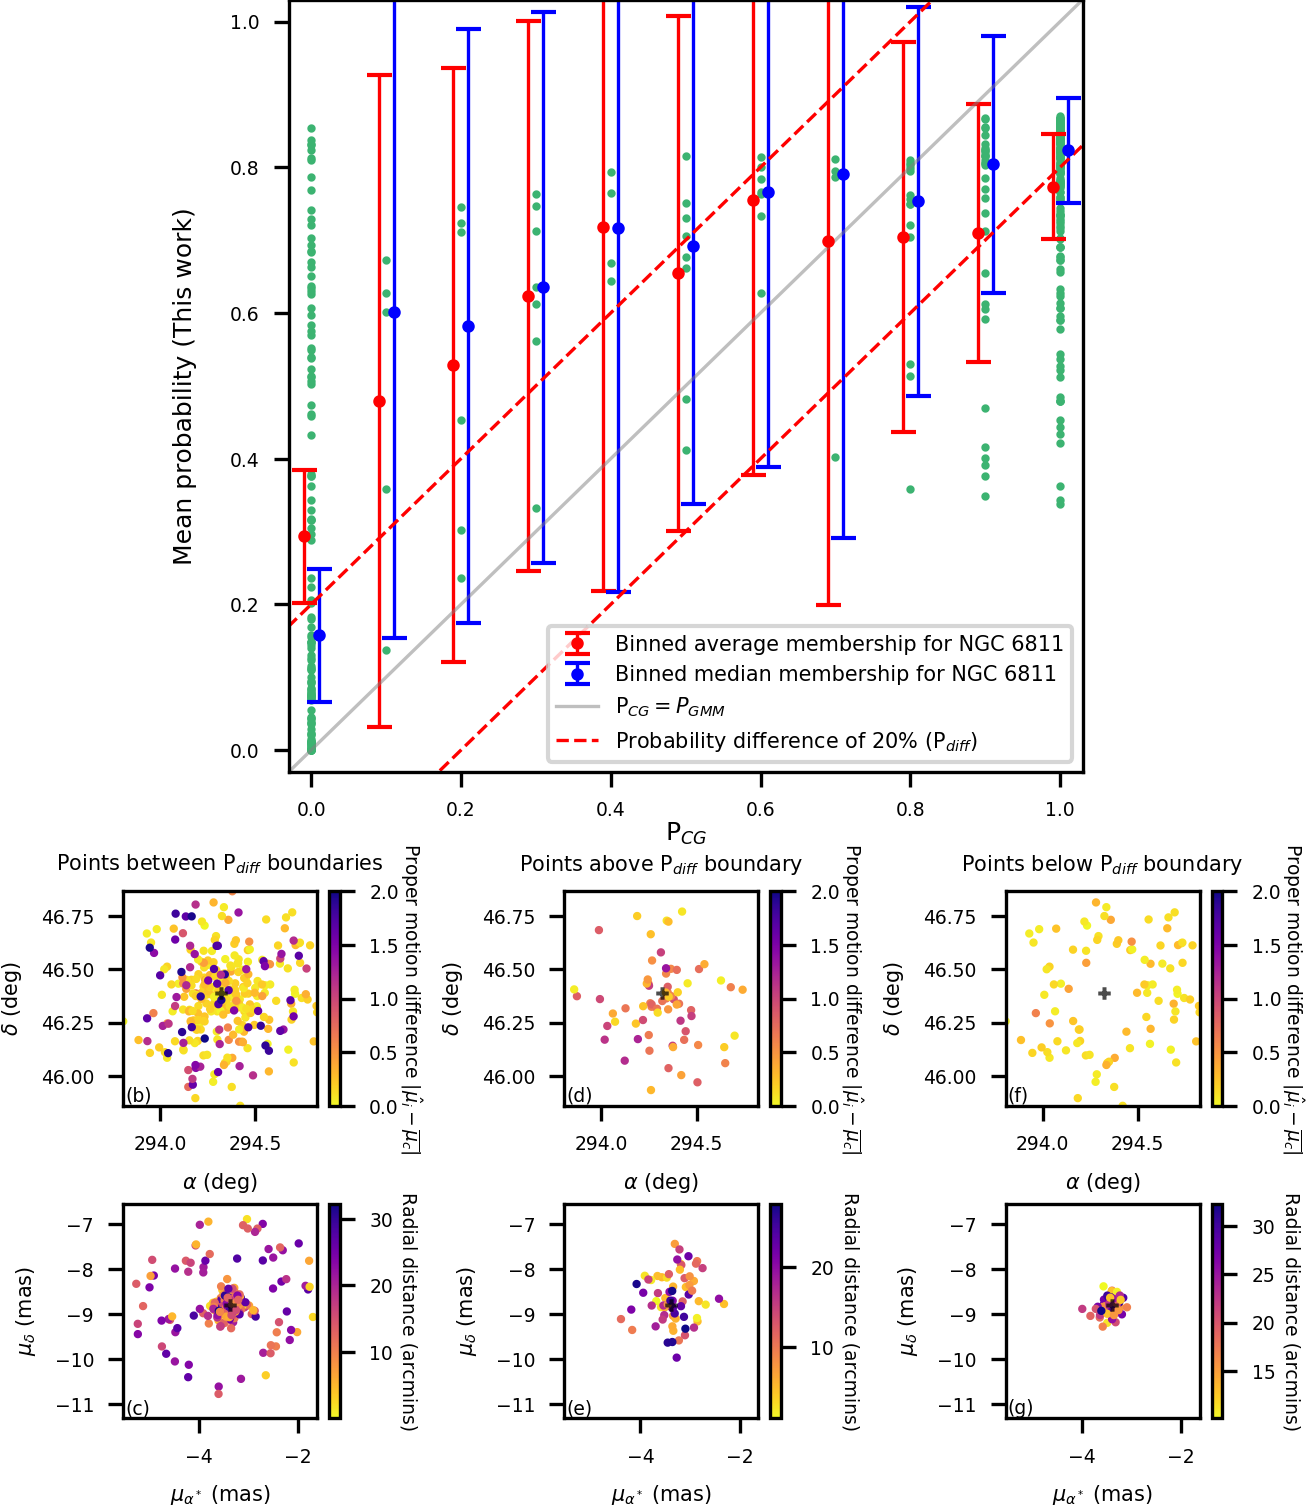
\includegraphics[width=\linewidth]{Chapter4/NGC6811_CG_comparison.png}
    \caption[Comparison of membership probabilities for NGC\,6811]{Same as Figure \ref{fig:CG_6791_comparison} but for NGC\,6811.}
    \label{fig:CG_6811_comparison}
\end{figure}

\begin{figure}[hbtp]
    \centering
    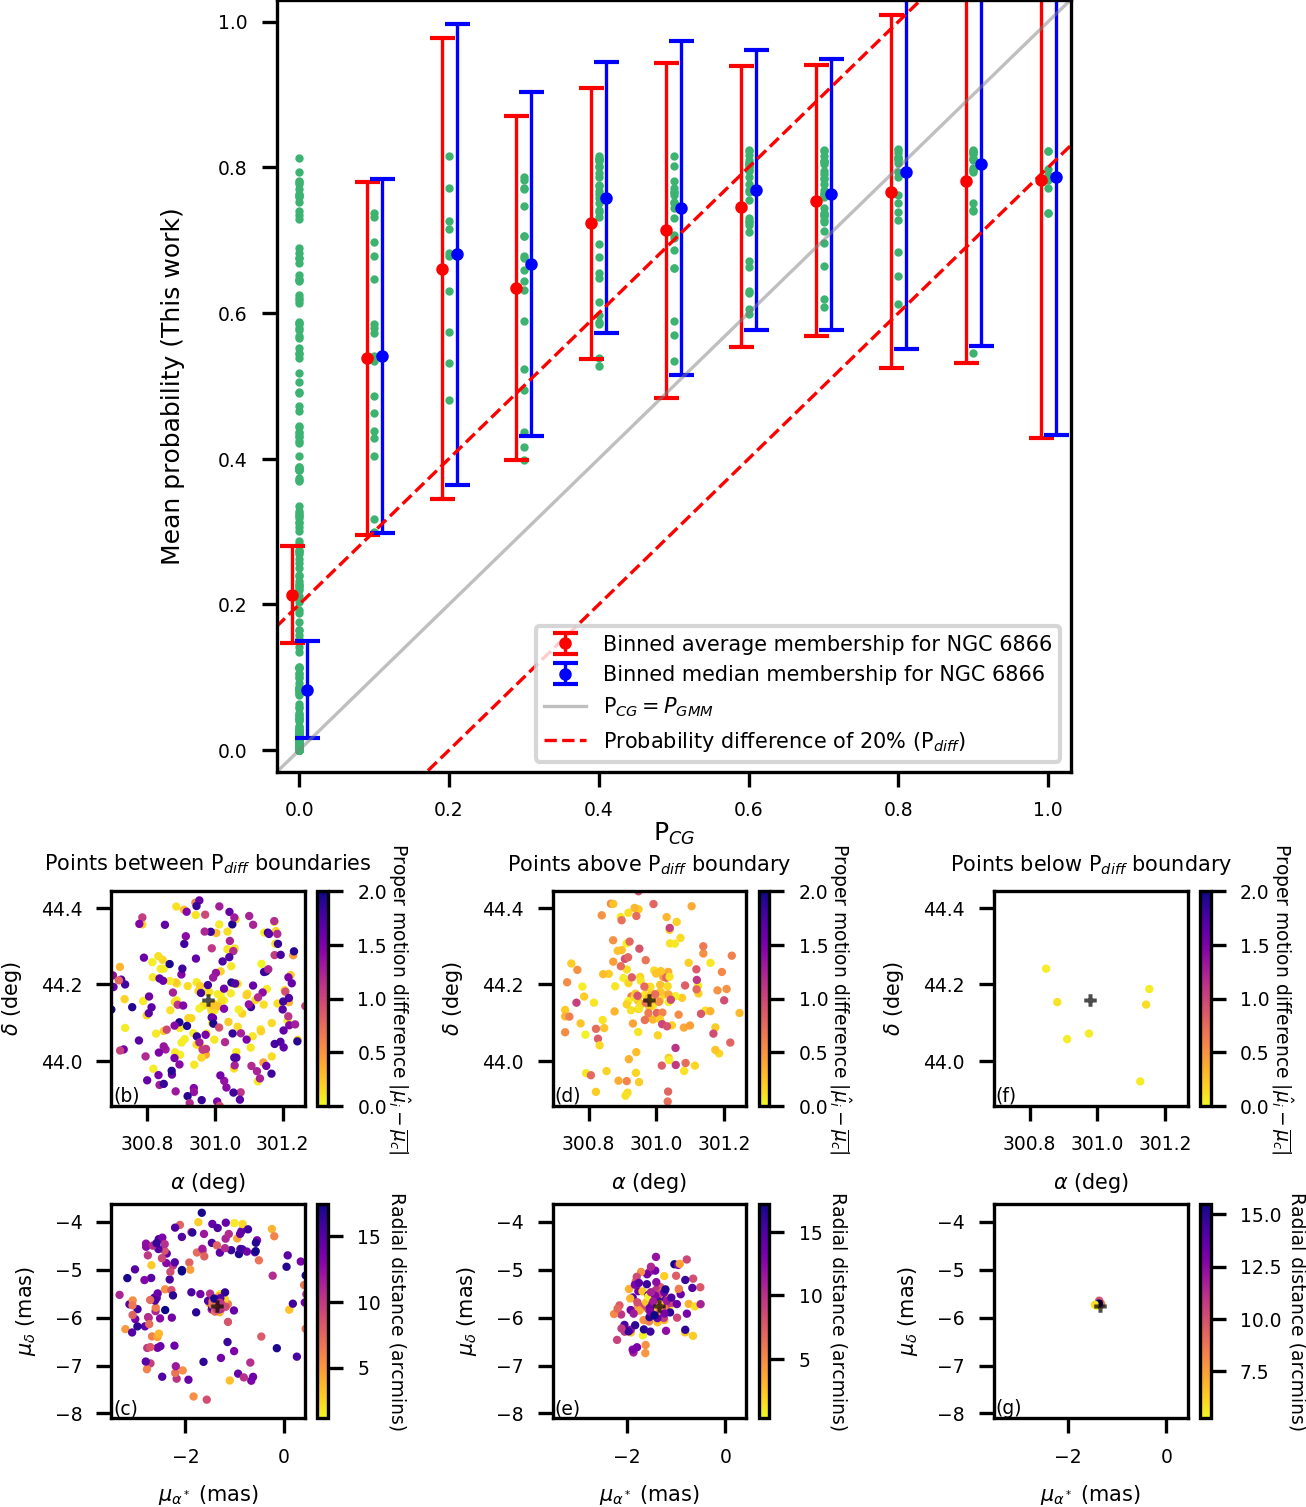
\includegraphics[width=\linewidth]{Chapter4/NGC6866_CG_comparison.png}
    \caption[Comparison of membership probabilities for NGC\,6866]{Same as Figure \ref{fig:CG_6791_comparison} but for NGC\,6866.}
    \label{fig:CG_6866_comparison}
\end{figure}

We inspected the relation between parallax, proper motion relative to the cluster, and the resulting membership scores derived in this work and CG18 for NGC\,6811 and NGC\,6866 (Figures \ref{fig:parallax_effect_6811} and \ref{fig:parallax_effect_6866}, respectively). It is clear from these figures that the inclusion of parallax in the clustering algorithm used by CG18 is the main reason for these lowered membership probabilities. They also appear to have a more strict density cutoff for proper-motion derived membership than that applied by our Gaussian kernel. The denser population of NGC\,6866 in parameter space, compared to NGC\,6811, also appears to have impacted CG18's analysis, leading to much higher membership values for these stars. Further investigation into these differences is beyond the scope of this thesis, but future work should include investigations into the effect of different field star densities, as well as simulating subsets of stars with parameters that are both similar and different to the average cluster member values, to identify the effects of deviations within the clustering parameters.

\begin{figure}[tpb]
    \centering
    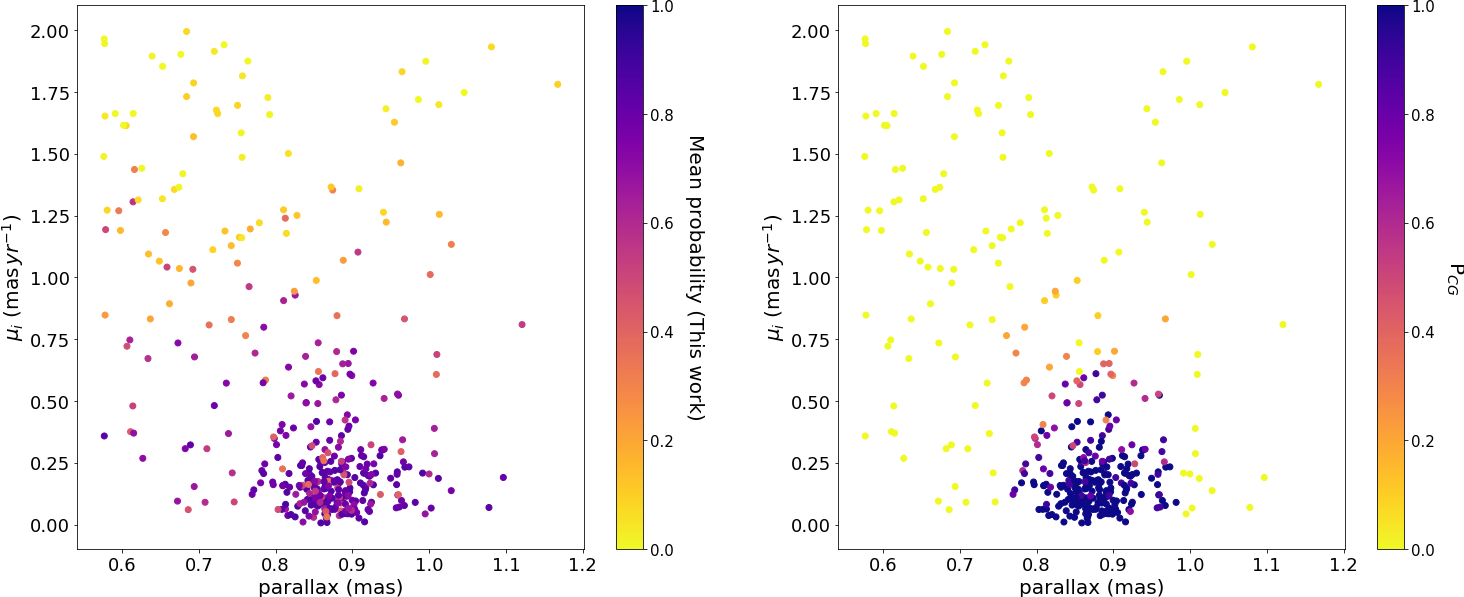
\includegraphics[width=\linewidth]{Chapter4/NGC6811_CG_comparison_parallax_all.png}
    \caption[Impact of parallax inclusion in membership analysis - NGC\,6811]{Relationship for NGC\,6811 between the parallax, and proper motion of stars relative to the cluster mean, colour-coded by the membership values from this work (left) and CG18 (right).}
    \label{fig:parallax_effect_6811}
    \vspace{0.5cm}
    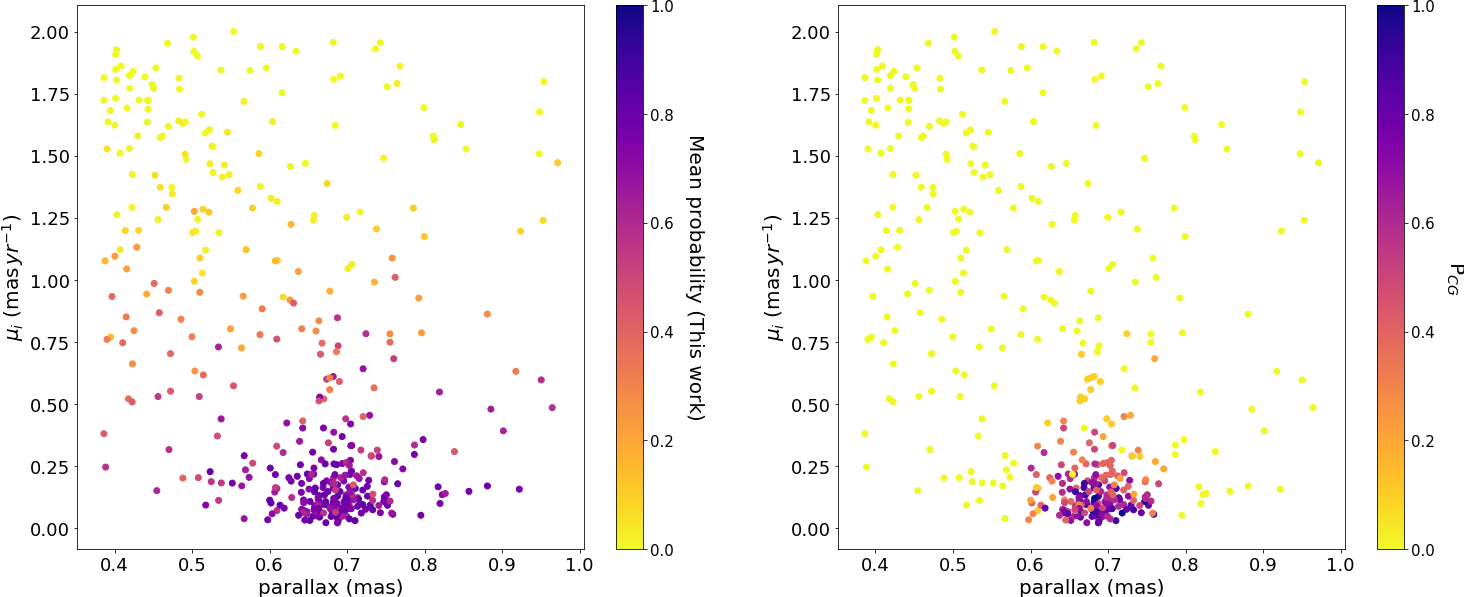
\includegraphics[width=\linewidth]{Chapter4/NGC6866_CG_comparison_parallax_all.png}
    \caption[Impact of parallax inclusion in membership analysis - NGC\,6866]{Same as Figure \ref{fig:parallax_effect_6811} but for NGC\,6866.}
    \label{fig:parallax_effect_6866}
\end{figure}

\subsection{WIYN Open Cluster Survey (WOCS) RV memberships}

The WIYN open cluster survey \citep{mathieu_wiyn_2000} has determined radial velocity (RV) membership probabilities for a limited subset of stars within both NGC\,6791, with 280 published values \citep{tofflemire_wiyn_2014} and NGC\,6819, with 1207 published values \citep{hole_wiyn_2009}. These membership probabilities were calculated by fitting two 1-D Gaussians to the stellar radial velocities within the cluster regions, and finding the relative heights between the field stars and cluster distributions. We used Simbad \citep{wenger_simbad_2000} to conduct the cross-match between Gaia DR2 IDs and WOCS IDs, and only selected stars common to both analyses where the corresponding WOCS survey classified the star as a single member (P $>$ 50\%). We chose this criteria to exclude binary systems that are potentially misclassified by our membership analysis, and to identify any situations where our membership did not correspond to those classified by other surveys as high confidence members. 

We identified 84 stars that fit this criteria for NGC\,6791 and 365 for NGC\,6819. In NGC\,6791 only 5 of these stars fell into our likely non-member classification with a membership score below 0.03. We note that one star with a score just above 0.2 in our membership did appear to lie outside the mean cluster proper motions from this common sample, and is potentially a non-member that has a higher membership score than our cutoff due to its position almost directly in the cluster centre. Figure \ref{fig:6791_wocs} shows the comparison between these RV membership probabilities and our membership determinations for NGC\,6791 (top left) with our likely non-members (red) and likely members (blue) shown relative to the overall distribution of positions (top right) and proper motions (bottom) for all stars within the cluster region (grey). The outlier with a mean membership score just greater than 0.2 is highlighted (black circle). In NGC\,6819 we found 138 stars classified as members by \citet{hole_wiyn_2009} but with low membership scores from our analysis. A comparison of these stars reveals this disagreement is present only for stars where the proper motion does not match the mean cluster values (Figure \ref{fig:6819_wocs}). 

\begin{figure}[hbtp]
    \centering
    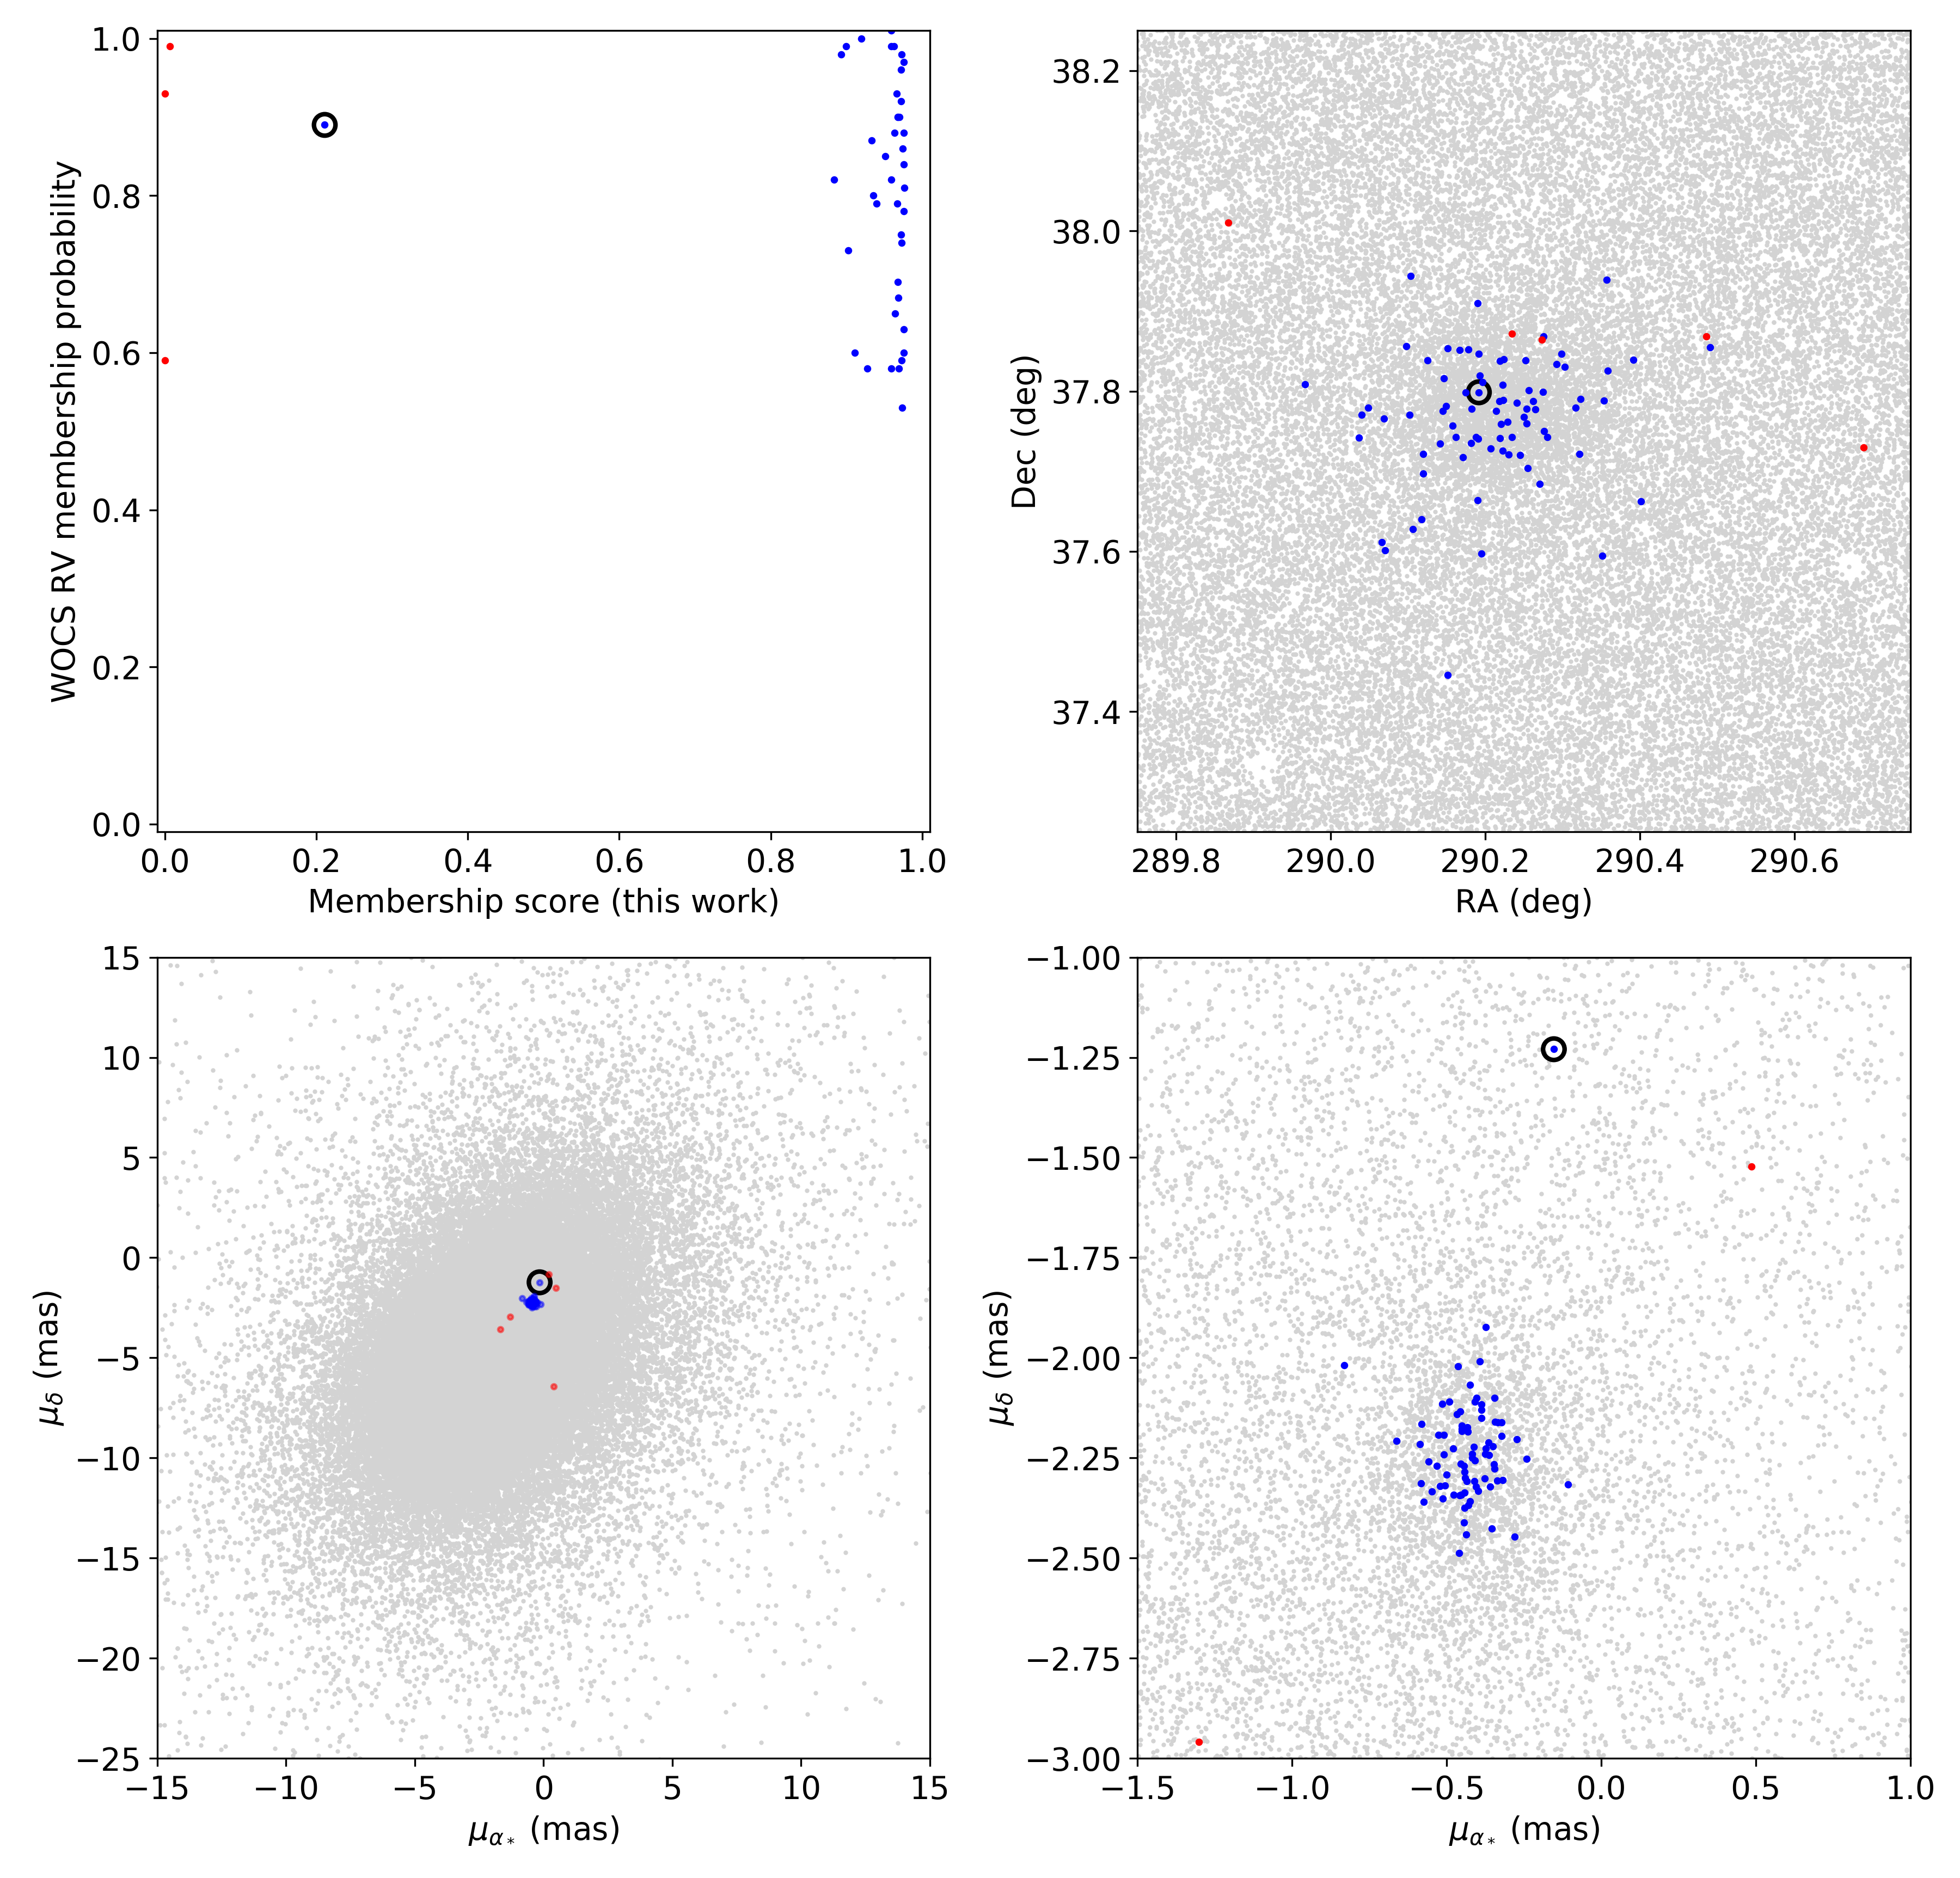
\includegraphics[width=0.98\linewidth]{Chapter4/wocs_com_6791.png}
    \caption[Comparison with WOCS RV members for NGC\,6791]{Comparison of membership probabilities between \cite{tofflemire_wiyn_2014} single cluster radial velocity members and this work for commonly investigated stars in NGC\,6791 (top left) with our likely non-members (red) and likely members (blue) shown relative to the overall distribution of positions (top right) and proper motions (bottom) for all stars within the cluster region (grey). One outlier with a mean membership score just greater than 0.2 is highlighted (black circle).}
    \label{fig:6791_wocs}
\end{figure}

\begin{figure}[hbtp]
    \centering
    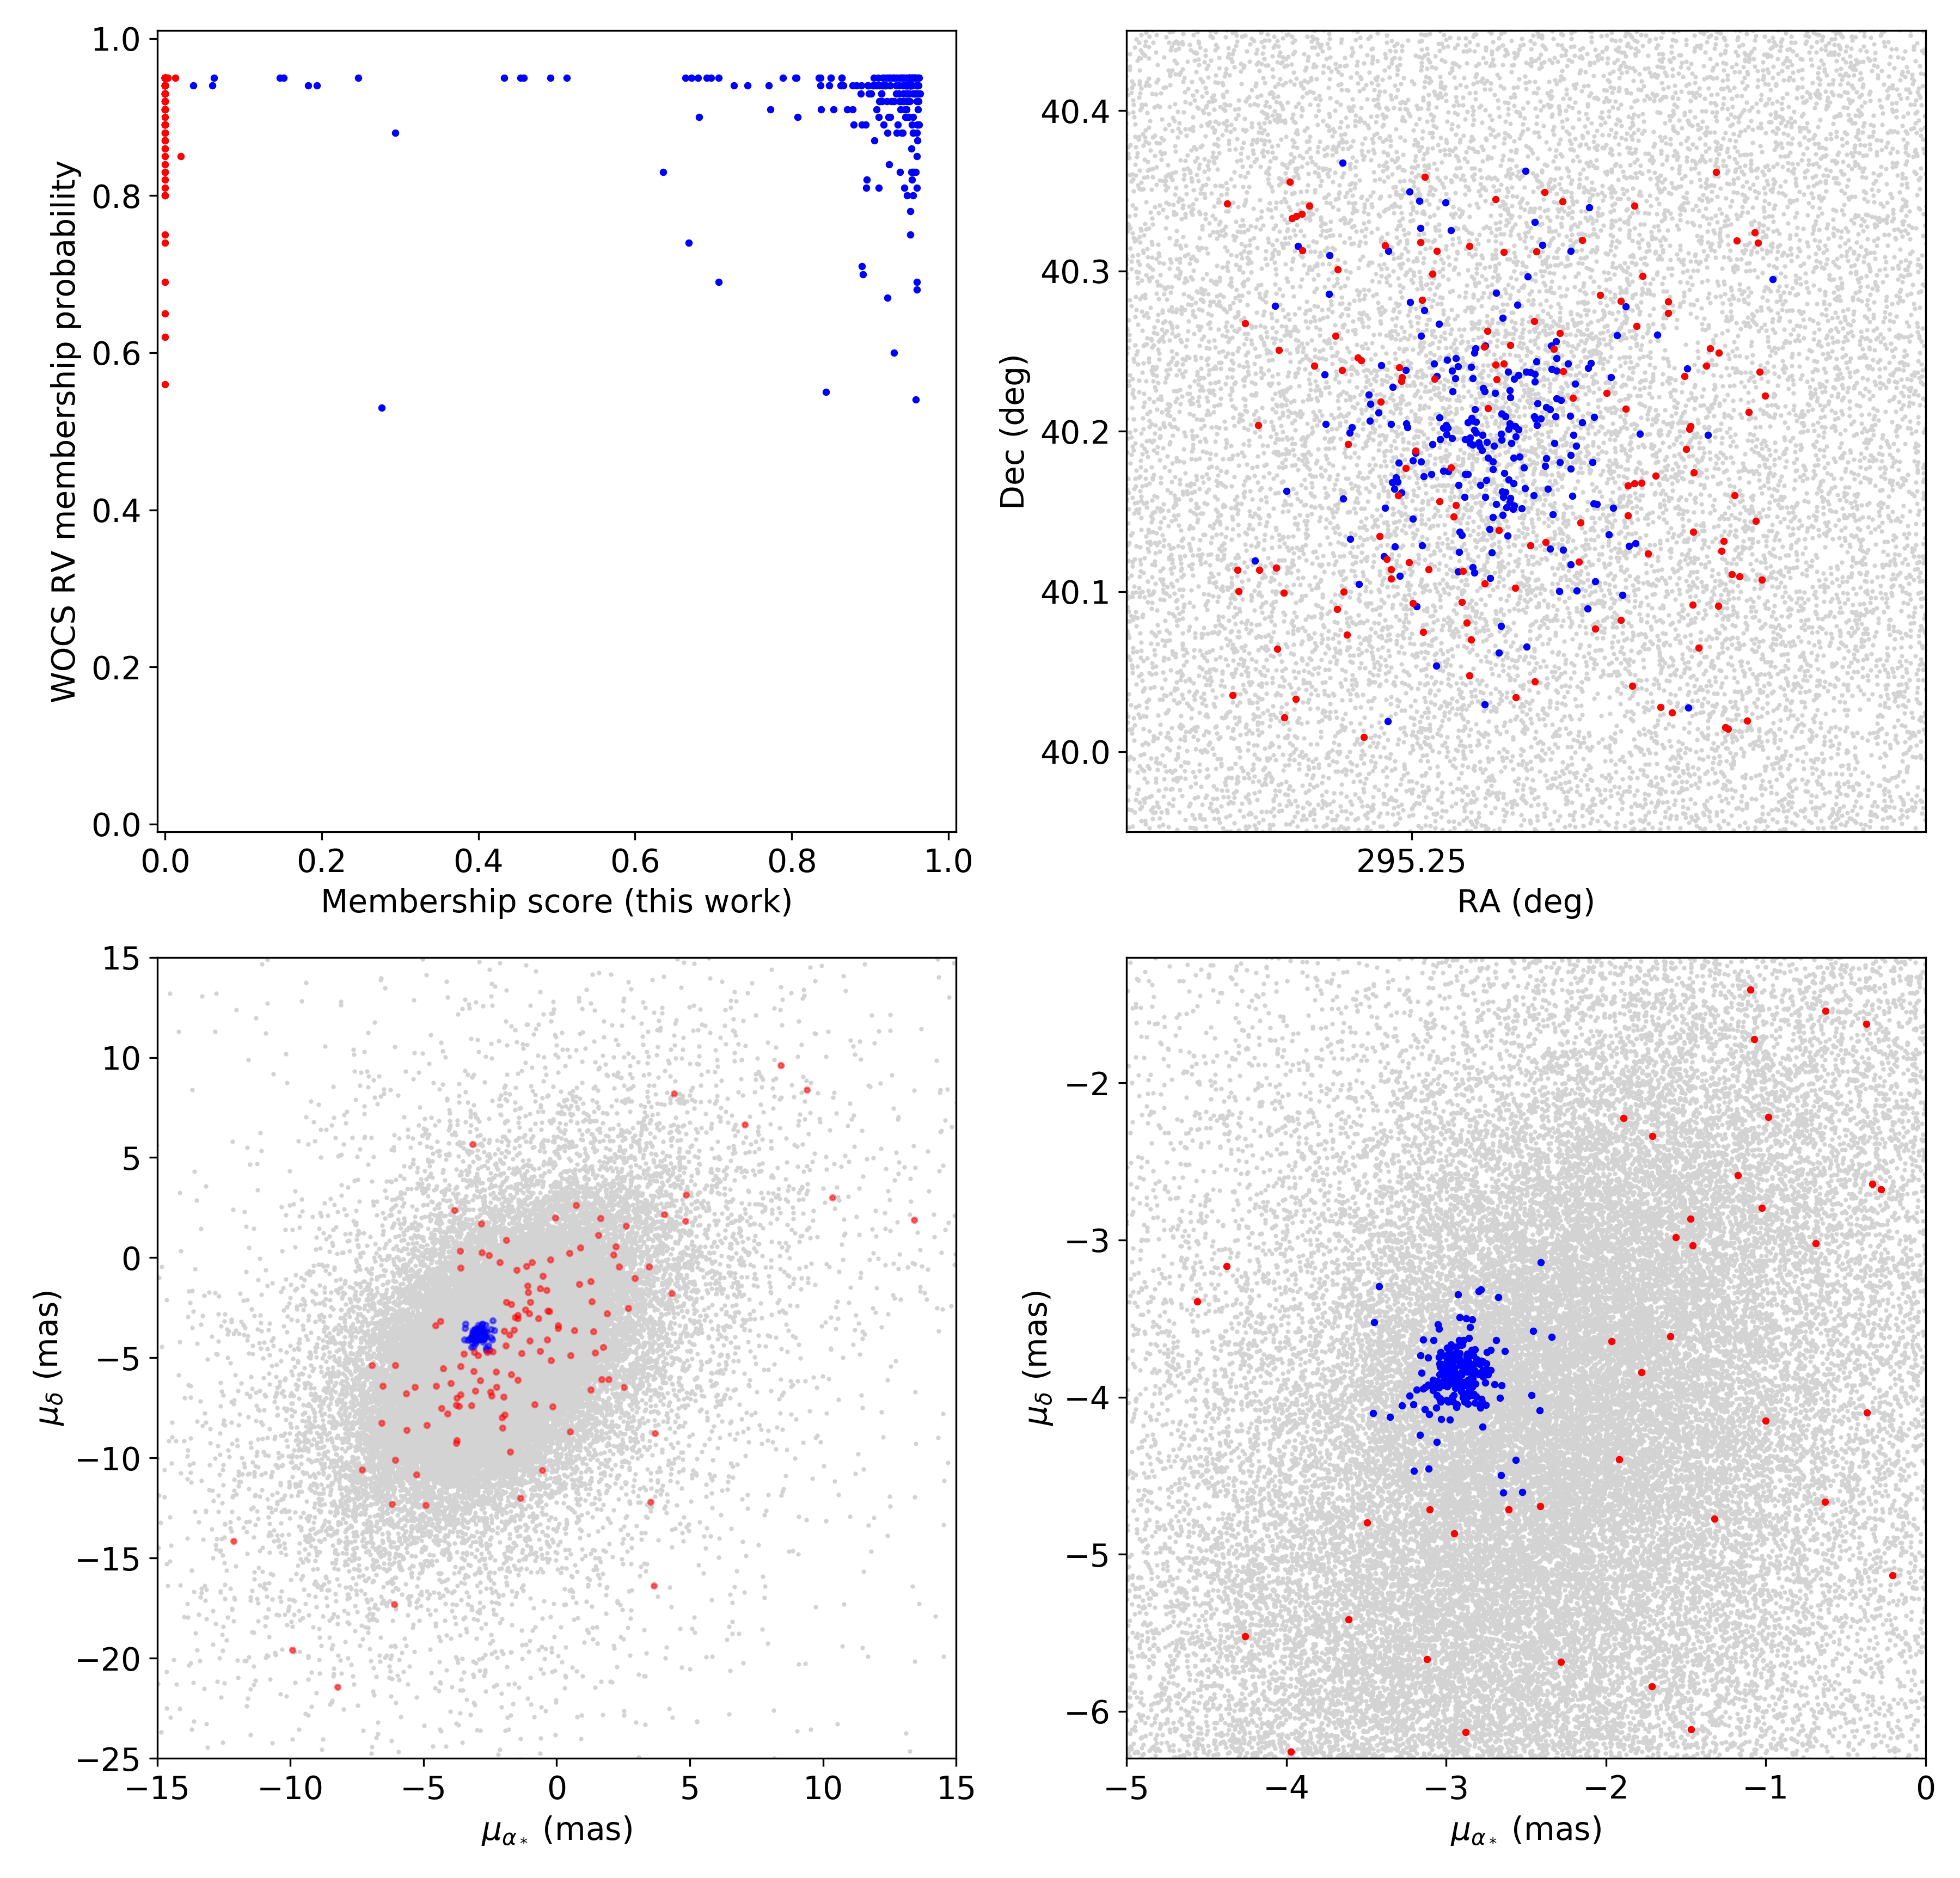
\includegraphics[width=0.98\linewidth]{Chapter4/wocs_com_6819.png}
    \caption[Comparison with WOCS RV members for NGC\,6819]{Same as Figure \ref{fig:6791_wocs} but for the comparison between \cite{hole_wiyn_2009} single cluster radial velocity members and this work for commonly investigated stars NGC\,6819.}
    \label{fig:6819_wocs}
\end{figure}

\subsection{Comparison conclusions}

Our Gaussian mixture modelling enables cluster membership to be determined as a fractional value based on the likelihood that a star belongs to one population or another. This allows us to account for both field stars and cluster stars in a single sample to large angular extents, while the Monte-Carlo simulation accounts for the heteroskedastic uncertainty parameter space of the \Gaia~DR2 data set.

Our comparison with the recent membership work by \cite{cantat-gaudin_gaia_2018} using the same dataset shows a mostly similar membership sample. The differences can be attributed to the inclusion of parallax values by CG18 for the closer clusters, the inclusion of field star populations in our mixture model, as well as the edge effects of the Gaussian kernels used in our membership analysis. CG18 analysed the entire \Gaia{} dataset to determine cluster memberships for the whole sky. Whilst the inclusion of parallax in CG18's clustering analysis is beneficial for clusters with well defined parallax values, in the case of these more distant clusters, the approach poses concerns. In particular, the uncertainty on the parallax values is of order the values themselves, and sampling this uncertainty parameter space will result in prior-dominated membership values. 

In addition, the CG18 analysis, whilst better suited for searching the entire sky for clusters, given the enormity of the data set and speed of analysis, only considers the field star distribution when sampling the uncertainty parameter space to ensure a cluster-like over density is present. Our analysis meanwhile includes this field star density when calculating the membership probability. The significantly increased number of MC iterations provides a more rigorous exploration the uncertainty parameter space (a factor of 100 times), which, combined with our inclusion of differing densities of the field population component between clusters closer to the galactic plane and those further away, and the prior dominated parallax inclusion in CG18's analysis for these more distant clusters, leads us to conclude that our method determines these cluster members in a more reliable manner than the k-means minimal spanning tree.

We note that our cluster membership determination is affected by the sharp cutoff of the edges of the Gaussian kernels. This edge effect artificially lowers the membership score for stars that are probable members located at the edge of the cluster. This kernel effect is avoided in the spanning tree model used by CG18. For future work it would be worthwhile investigating a mixture model analysis using more accurate cluster models for the parameter spaces, such as isothermal elliptical kernels in spatial dimensions \citep{kuhn_mixture_2017}, and the inclusion of a constant offset model along with two bi-variate Gaussian kernels for the proper motion dimensions. In addition, our membership score does not easily translate to a statistical probability of membership and it would be ideal to determine a method of normalising these membership scores, perhaps using a logistic regression function.

Our comparison with the more limited radial velocity membership from the WIYN open cluster survey (WOCS) reveals that our membership scores match well with their complementary and independent radial velocity memberships. For those stars where our memberships disagree with those of \citet{tofflemire_wiyn_2014} and \citet{hole_wiyn_2009}, the proper motions from \Gaia{} show large differences from the mean cluster value. As such these stars represent foreground or background non-members that have similar radial velocities to the cluster population.

\section{Kepler-Gaia DR2 Cross-matching}

To combine this membership analysis with the photometric (and thus asteroseismic) \Kepler~information, we need to match the \Kepler~and \Gaia~identifiers.

\citet{berger_revised_2018} produced a \Gaia~cross-matched database for all \Kepler~targeted stars to allow for astrometric analysis of these stars, but excluded non-targeted cluster stars. \cite{colman_pixels_2020} have now extracted light curves for many of these non-targeted stars within the centres of the open clusters from the \Kepler~superstamps. %(\todo{citation}Colman et al. (2019, in prep.),\, %\citet{Colman19}, 
%Ch. \ref{chap:lightcurves}). 
These stars are now of particular interest in terms of cluster membership for conducting ensemble asteroseismic analyses, and require a cross-match between \Kepler~and \Gaia~identifiers.

% Before cross-matching the \Gaia~and \Kepler~catalogs, we converted the Gaia stellar positions ($\alpha$, $\delta$) from the J2015.5 reference frame to the J2000.0 reference frame used by the \Kepler~Input Catalog (KIC) \citep{brown_kepler_2011}. 
Before cross-matching the \Gaia~and \Kepler~catalogs, we corrected the Gaia stellar positions ($\alpha$, $\delta$) for proper motion to the J2000.0 epoch. We then restricted the cross-match to stars within a radius of each cluster centre equal to the angular size used for our membership analysis (see \cref{tab:cluster_selection}).

To begin the cross-match, we removed all KIC stars without a \Kepler~magnitude (Kp). For every \Gaia~star, we selected all matches within an initial 3\,arcsecond radius. We further filtered the matches by imposing a magnitude cut based on the \Gaia~G-band photometry and \Kepler~magnitude to ensure ${|G-K\mathrm{p}| \leq 2}$, and selected the closest star as the best match. We selected this magnitude cutoff to minimize scatter in the \Kepler-\Gaia CMD for stars of all evolutionary stages. Figure \ref{fig:KGcmd} reveals a tight relation between the $G$ and $K_\mathrm{p}$ magnitudes for the red giant and red clump stars, with greater scatter around the main sequence stars and turn-off. For any duplicate \Kepler~matches we selected the \Gaia~match with the smallest angular separation. We then removed this \Kepler~match from the possible matches, and iteratively repeated the cross-match until all stars were matched or no further match was found. 

\begin{figure}[htb]
    \centering
    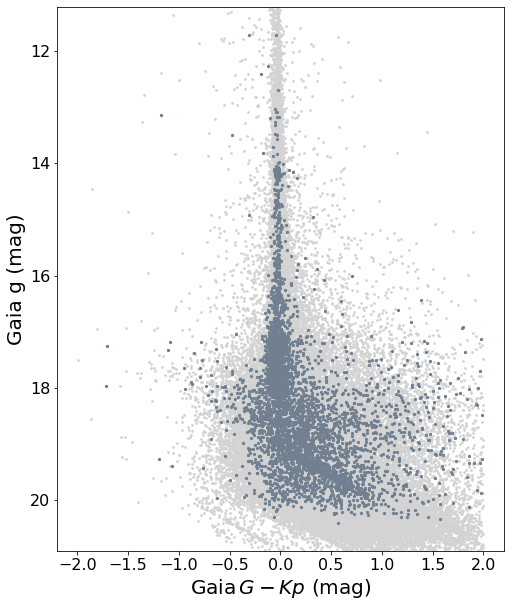
\includegraphics[scale=0.5]{Chapter4/kic_gaia_photometric_comparison.png}
    \caption[Gaia-Kepler colour magnitude diagram]{Gaia-Kepler Colour-magnitude diagram. Field stars (light grey) and cluster stars (dark grey) show a tight relation for the red giant and red clump stars, with greater scatter apparent for the main sequence stars.}
    \label{fig:KGcmd}
\end{figure}

Finally, we inspected the angular separations of all the matches %(Figure \ref{fig:angsep_matches}) 
and removed any with angular separations greater than 1.5 arcseconds. We selected this separation based on a fit to a transformed Poisson distribution capturing 95\% of the total matches. As suggested by \citet{berger_revised_2018}, we assumed any matches beyond this angular separation were likely to be spurious background or foreground contaminants. We joined this cross-matched database with our GMM values to form our final database of cross-matched cluster stars with membership scores. 

% \begin{figure}
%     \centering
%     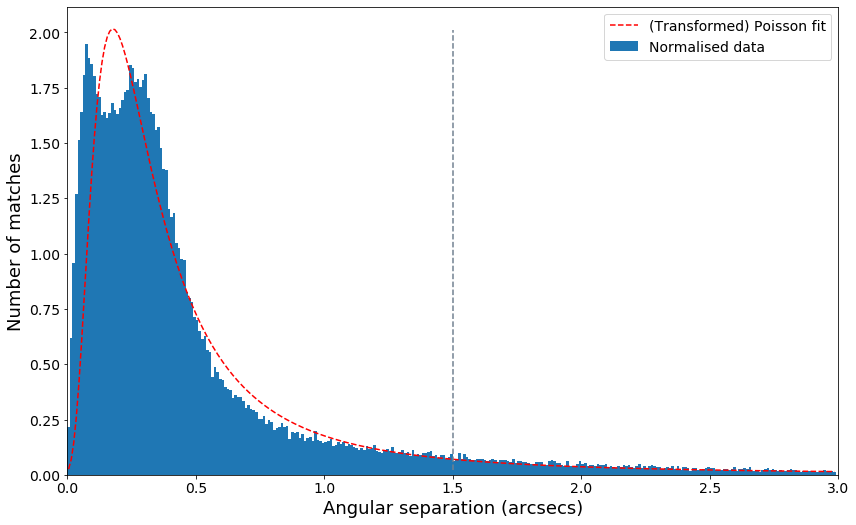
\includegraphics[scale=0.5]{Chapter4/crossmatch_angsep.png}
%     \caption[Histogram of angular separations for cross-matches.]{Histogram of the angular separations for all cross-matches. A transformed Poisson distribution (red curve) and the 95\% cumulative count (dashed vertical line) highlight the criteria used in separating spurious field contaminants from true matches.}
%     \label{fig:angsep_matches}
% \end{figure}

\label{sect:cuts}

For our GMM probability determination, we used a radial distance cut from the cluster centres based on the J2015.5 reference epoch of the \Gaia~DR2 database. As a result of stellar proper motion, a few of the stars at the edges of these radial distance cuts are either not present in the GMM membership determination, or not present in the cross-match database. These stars are all likely to be non-members based on their distance from the cluster centre. We present the number of stars included at each stage of the cross-match, for each cluster field of view, in Table \ref{tab:cluster_crossmatch}. 

Extracts of the completed cross-match databases for all four open clusters, showing the 60 highest mean probability cluster members, are presented in Tables \ref{tab:6791mem} - \ref{tab:6866mem}. The complete databases are available online\footnote[2]{https://jason-drury.github.io/}. These tables will be useful for future studies of these clusters. In the next chapter we investigate the cluster red giant members, and compare these astrometric memberships with the comparable asteroseismic membership determinations.

\begin{table}[p]
    \centering
    \setlength\tabcolsep{11pt}
    % \renewcommand{\arraystretch}{1.25}
    \begin{tabular}{lcccc}
        \toprule
         & NGC\,6791 & NGC\,6819 & NGC\,6811 & NGC\,6866 \\
        \midrule
        \midrule
        Database (radial cut) &  &  &  & \\
         - Gaia  & 153626 & 137584 & 29004 & 17841 \\
         - Kepler& 126866 & 88602 & 25168 & 10078 \\\rule{-3pt}{1.2em}
        Stars with Kepler & \multirow{2}{*}{125018} & \multirow{2}{*}{86831} & \multirow{2}{*}{24724} & \multirow{2}{*}{9829} \\
        magnitudes ($K_p$) &  &  &  & \\\rule{-3pt}{1.2em}
        Target light & \multirow{2}{*}{2404} & \multirow{2}{*}{3372} & \multirow{2}{*}{1215} & \multirow{2}{*}{397} \\
        curves available &  &  &  & \\\rule{-3pt}{1.2em}
        Cross-matches & 109916 & 80531 & 21318 & 9407 \\\rule{-3pt}{1.2em}
        Cross-matches & \multirow{2}{*}{103318} & \multirow{2}{*}{75368} & \multirow{2}{*}{19679} & \multirow{2}{*}{8832} \\
        (ang. sep. $\leq$ 1.5\,arcsec) &  &  &  & \\\rule{-3pt}{1.2em}
        Final database with & \multirow{2}{*}{102890} & \multirow{2}{*}{74866} & \multirow{2}{*}{19616} & \multirow{2}{*}{8769} \\
        GMM memberships &  &  &  & \\\midrule
        \rule{-3pt}{1.2em}
        Difference & 428 & 502 & 63 & 63 \\\midrule
        \rule{-3pt}{2em}
        Likely members: &  &  &  & \\\rule{-3pt}{1.2em}
         - Mean posterior & \multirow{2}{*}{0.03} & \multirow{2}{*}{0.03} & \multirow{2}{*}{0.05} & \multirow{2}{*}{0.05} \\
           membership cut &  &  &  & \\\rule{0pt}{1em}
         - Stddev posterior & \multirow{2}{*}{0.3} & \multirow{2}{*}{0.3} & \multirow{2}{*}{0.15} & \multirow{2}{*}{0.15} \\
           membership cut &  &  &  & \\\rule{0pt}{1em}
         - Mean prob. & 4424 & 3554 & 1296 & 868 \\\rule{-3pt}{1.2em}
         - Stddev. cut & 3590 & 3275 & 777 & 507 \\\rule{-3pt}{1.2em}
         - Distance cut & 2388 & 3254 & 393 & 483 \\\rule{-3pt}{1.2em}
         - In superstamp & 1437 & 1244 & -- & -- \\\rule{-3pt}{1.2em}
         - Not targeted & 1327 & 1047 & 203 & 379 \\\rule{-3pt}{1.2em}
         - Partial mission target & 8 ($\leq$ 8 Qs) & 155 ($\leq$ 14 Qs) & -- & -- \\\rule{-3pt}{1.2em}
         - Full mission target & 110 & 177 & 190 & 104 \\
        \bottomrule
    \end{tabular}
    \caption[Number of stars present in the cross-matched database at each stage]{Number of stars present in the cross-matched database at each stage. The top rows list the initial number of stars within the cluster radius for the Kepler Input Catalog (KIC) and the Gaia DR2 catalog. The total number of cross matches is followed by the number remaining after likely contaminants are removed, based on a maximum angular separation of 1.5\,arcsecs. The number of stars with GMM membership scores is listed, with the difference between these two numbers underneath. The number of stars with membership scores differs slightly from the cross match as the latter includes proper motion corrections for stellar positions. The stars that are different are all located at the edge of the selected radius, beyond the cluster radii, and will be non-members. The values selected for the mean and standard deviation cuts within the cluster membership distributions are shown, followed by the number of likely members after each cut is made. An additional distance cut removes any stars that have serendipitously similar proper motions to the mean open cluster motion. This row shows the number of stars in our final cluster membership determination.}
    \label{tab:cluster_crossmatch}
\end{table}

%Could not use APASS gri photometry to fill in Kepler data and generate predicted G mag as Berger due to cluster members typically being much fainter than the limiting cutoff mag for APASS.

% For stars with multiple matches that satisfied these criteria, we decided to keep those with the smallest angular separations. Of the 197,104 stars present in the KSPC, we identified Gaia DR2 source matches for 195,710. Stars with poorly determined parallaxes (σ π /π > 0.2), low effective temperatures based on our adopted values (T eff < 3000 K, see Section 2.2), extremely low log g (< 0.1 dex), and/or non-“AAA”-quality Two Micron All Sky Survey (2MASS) photometry were rejected from our sample.

% Additionally, we made astrometric cuts similar to those described in Appendix C of Lindegren et al. (2018) and Section 4.1 of Arenou et al. (2018). In particular, we used Equation (1) (unit weight error compared to a function of the G magnitude of the source that helps filter contamination from binaries and calibration problems) and Equation (3) (greater than eight groups of observations separated by at least 4 days) of Arenou et al. (2018) to remove stars with bad astrometric solutions. We did not use the astrometric excess noise values provided by Gaia DR2 to filter stars because they were less discriminating for stars with G < 15 due to the “degree of freedom bug” (see Appendix A and C of Lindegren et al. 2018). We did not use Equation (2) of Arenou et al. (2018), a cut ensuring that Gaia has clean photometry of the included sources, because we utilized separate 2MASS photometry in our analysis. As discussed in Lindegren et al. (2018), our imposed cuts removed many stars that appear in unphysical areas of radius-T eff parameter space, such as the “subdwarfs” between the stellar main sequence and the white dwarf branch. Excluding these stars reduced our final sample to 177,911 Kepler stars.

% \newpage
% \subsection*{Declaration}
% The work presented in this chapter was conducted in conjunction with my supervisors Dennis Stello and Tim Bedding who provided suggestions and feedback on the analysis as it proceeded.
